\documentclass[12pt]{article}
\usepackage[utf8]{inputenc}
\usepackage{amsmath, amssymb}
\usepackage{geometry}
\usepackage{graphicx}
\usepackage{lmodern}
\usepackage{float}
\usepackage[russian]{babel}
\usepackage{caption}
\usepackage[most]{tcolorbox}
\usepackage{amsfonts}

\geometry{a4paper, margin=2.5cm}
\newcommand{\ri}[1]{\mathrm{#1}\kern-0.1em}

\title{Решение обратной задачи термометрии}
\author{}
\date{}

\begin{document}

\maketitle

\section*{Модель распределения температуры в скважине}

Ранее были получены аналитические решения о равновесном распределении по глубине \( z \) действующей
нагнетательной скважины средней по ее поперечному сечению температуры \(\langle \theta \rangle\)
для двух типов участков, изолированных от пласта:

\begin{enumerate}
    \item проточного \(-\langle \theta_{\ri{I}} \rangle (z; \text{Ре, А})\);
    \item застойного (завершающего) \(-\langle \theta_{\ri{II}} \rangle (z; \text{A})\).
\end{enumerate}

Среднюю в поперечном сечении \( z \) ствола скважины температуру \(\langle \theta \rangle\)
в дальнейшем для простоты будем называть температурой в точке \( z \). Общее равновесное распределение температуры вдоль
ствола скважины, имеющей гидродинамическую связь с пластом, ранее приближалось с помощью указанных двух типов решений,
в предположении о том, что протяженность интервалов оттока жидкости в пласт много меньше расстояния между ними, и они могут
быть заменены сосредоточенными стоками. В этом случае общее решение является кусочно-непрерывной функцией,
составленной из функций вида \(\langle \theta_{\ri{I}} \rangle\) со скачком параметра Pe
при переходе через каждый точечный сток на величину, соответствующую интенсивности оттока,
с завершением функцией вида \(\langle \theta_{\ri{II}} \rangle\) на застойном участке.

Расширим условия приближенной модели -- поскольку в состоянии, близком к равновесному,
температура в стволе скважины на интервалах поглощения будет слабо меняться вдоль координаты \( z \)
ввиду малого радиального градиента температуры жидкости, проникшей в пласт, то вдоль этих интервалов можно полагать
температуру в скважине постоянной: \(\langle \theta_{\ri{III}} \rangle = \text{const}\). Тогда можно записать более общую
запись приближенной непрерывной функции температуры вдоль ствола скважины, состоящего из чередующихся изолированных
интервалов и интервалов утечки и заканчивающегося застойным участком:

\[
\langle \theta \rangle(z) =
\begin{cases}
\langle \theta_{\ri{I}} \rangle(z; \text{Pe}; \text{A}), & z_{i,0} \leq z \leq z_{i,1}, i=1 \dots N-1; \\
\langle \theta_{\ri{III}} \rangle(z) = \langle \theta_{\ri{I}} \rangle(z_{i,1}; \text{Pe}; A), & z_{i,1} \leq z \leq z_{i+1,0}, i=1 \dots N-1; \\
\langle \theta_{\ri{II}} \rangle(z; \text{A}), & z_{N,0} \leq z \leq z_{N,1}. \\
\end{cases}
\]

Здесь \( N \) -- число изолированных участков ствола скважины на интервалах \([z_{i,0}, z_{i,1}]\),
из которых первые \( N-1 \) являются проточными, а последний под номером \( N \) является застойным.
Соответственно на интервалах \([z_{i,1}, z_{i+1,0}]\) расположены участки поглощения пластом закачиваемой жидкости.

\section*{Общая постановка обратной задачи}

Требуется идентифицировать количество изолированных участков скважины, координаты их расположения
$\{z_{i,0}, z_{i,1}\}_{i = 1 \dots N}$
и интенсивность интервалов утечки в пласт нагнетаемой в скважину воды по результатам термометрии
в действующей скважине, предполагая распределение температуры установившимся. Дебит скважины, её радиус,
теплофизические свойства пласта и крайние координаты ствола скважины $z_{1,0} = 0, z_{N,1} = L$
считаются известными. Интенсивность стока на каждом участке
поглощения пересчитывается в локальное число Пекле $\text{Pe}_i, i = 1 \dots N-1$.
Последний интервал считается непроницаемым и застойным: $\text{Pe}_N = 0$.

Таким образом, общее число неизвестных:
\[
3N - 3.
\]

С учетом наличия погрешности в замерах температуры, неточности в задании ТФС и других параметров системы,
а также самого приближенного решения перечисленные
неизвестные величины отыскиваются методом квазирешения путем минимизации функционала
уклонения :
\[
E(\theta) = \frac{1}{n} \sum_{j=1}^{n} \left( \langle \theta \rangle(z_j, \xi) - \langle \theta \rangle_j \right)^2 \rightarrow \min_{\xi} \tag{1}
\]

где:
\begin{itemize}
  \item $n$ — число замеров температуры вдоль ствола скважины;
  \item $\langle \theta \rangle_j$ — замеры температуры на глубине $z_j$;
  \item $\xi$ — полный набор неизвестных параметров задачи.
\end{itemize}

В качестве замеров температуры со скважины используются модельные данные с наложенным шумом: к каждому замеру
добавляется случайная величина~$\xi$, распределённая по нормальному закону: $\xi \sim \mathcal{N}(0, \sigma^2)$.
\section*{Разделение задачи на подзадачи}

\begin{enumerate}
    \item Отыскиваются точки роста сглаженной кривой, определяются количество и координаты участков утечки;
    \item Производится численная оптимизация для оценки интенсивности утечек.
\end{enumerate}

\section*{Алгоритм первой подзадачи}

При отсутствии шума в данных изолированные участки можно находить по производной: там, где она отлична от нуля, и будет находится изолированный участок.
При наличии шума производную невозможно исследовать напрямую, так как кривая имеет множество локальных пиков и впадин. Для такой задачи был написан алгоритм, основанный на скользящей оконной регрессии. Такой подход позволяет оценивать общий тренд роста кривой,
игнорируя локальные скачки. Для начала производится дополнительная нормировка графика:
\[
z_i^{\text{norm}} = \frac{z_i - \min(z)}{\max(z) - \min(z)}, \quad
\theta_i^{\text{norm}} = \frac{\theta_i - \min(\theta)}{\max(\theta) - \min(\theta)}
\]

Затем шумная кривая сглаживается медианным фильтром и по массиву сглаженных значений температуры проходится регрессия.

\begin{center}
    \includegraphics[width=0.85\textwidth]{intervals_3}
\end{center}

Проблема: параметры алгоритма (размер окна и угол наклона для регрессии) чувствительны к входным параметрам задачи: Pe, A, $\sigma$, $N$.
\textbf{Цель:} Написать алгоритм, который сам находит оптимальный набор параметров регрессии (далее гиперпараметров) для заданной комбинации входных параметров. Идея решения заключается в написании
ML модели, которая после обучения будет предсказывать оптимальные гиперпараметры. Для этого сначала нужно набрать обучающую выборку в формате:
\[
\text{Pe}_0,\ \text{A},\ \sigma,\ N,\ \text{window\_size},\ \text{min\_slope}
\]
Выборку будем набирать на примере выше.

Для каждой комбинации параметров, подающихся на вход, решается задача минимизации функционала ошибок MAE:
\[
\text{MAE} = \frac{1}{n} \sum_{i=1}^{n} \left| y_i(\theta) - \hat{y}_i \right| \rightarrow \min_{\theta} \tag{2}
\]

где:
\begin{itemize}
  \item $y_i(\theta)$, $\hat{y}_i$ — предсказанное моделью и истинное значение $i$-й границы изолированного участка;
  \item $\theta$ — вектор гиперпараметров задачи;
\end{itemize}

\section*{Далее есть два подхода для решения задачи (2)}

\section*{Подход 1: Поиск по сетке}

Создаются две сетки значений: одна для входных параметров, другая для гиперпараметров. Например, можно брать такие значения:
\begin{center}
    \includegraphics[width=0.85\textwidth]{/Users/macbookmike_1/Downloads/grid}
\end{center}

\begin{center}
    \includegraphics[width=0.85\textwidth]{/Users/macbookmike_1/Downloads/grid_@}
\end{center}

Перебираются все комбинации из первой сетки, для каждой такой комбинации перебираются параметры из второй сетки и выбираются оптимальные.
Оптимальные значения для каждой комбинации усредняются по $N_{\text{rnd}}$ реализациям шума. Вычислительная сложность такого подхода: $O(N_{\text{rnd}}*k^4*m*n)$, где ${k}$ - количество возможных значений для каждого входного параметра, $m, n$ - количество возможных значений для гиперпараметров.

\section*{Подход 2: Байесовская оптимизация}

Также фиксируется сетка входных параметров. Далее, вместо перебора гиперпараметров, применяется байесовская оптимизация. Строится вероятностная модель (гауссовский случайный процесс) приближения функционала (2). Вместо минимизации $E(\theta)$ используется функция ожидаемого улучшения (Expected Improvement):

\[
EI(x) = (f_{best} - \mu(x)) \Phi(Z) + \sigma(x) \phi(Z), \quad Z = \frac{f_{best} - \mu(x)}{\sigma(x)} \tag{3}
\]

Где:
\begin{itemize}
    \item $f_{best}$ — текущее минимальное значение (2);
    \item $\mu(x), \sigma(x)$ — аппроксимированные среднее и стандартное отклонение в точке $x$;
    \item $\Phi$ и $\phi$ — функции распределения и плотности нормального распределения.
\end{itemize}

На каждой итерации выбирается новая точка $x$, максимизирующая $EI(x)$. С каждой итерацией модель всё точнее
описывает поведение функционала (2), направляя поиск в наиболее вероятные положения минимума.
Число итераций, то есть вызов функции (3) задается заранее, до начала работы алгоритма.
Зачастую берётся 50 итераций как компромисс между качеством и временем. Вычислительная сложность такого подхода:
 $O(N_{\text{rnd}}*k^4*50)$, что значительно меньше простого перебора.

\begin{center}
    \begin{minipage}{0.48\textwidth}
        \includegraphics[width=\linewidth]{/Users/macbookmike_1/Desktop/bayes_animation it_1}
    \end{minipage}
    \hfill
    \begin{minipage}{0.48\textwidth}
        \includegraphics[width=\linewidth]{/Users/macbookmike_1/bayes_animation it_15}
    \end{minipage}
\end{center}

\begin{center}
    \begin{minipage}{0.48\textwidth}
        \includegraphics[width=\linewidth]{/Users/macbookmike_1/bayes_animation it_30}
    \end{minipage}
    \hfill
    \begin{minipage}{0.48\textwidth}
        \includegraphics[width=\linewidth]{/Users/macbookmike_1/bayes_animation it_50}
    \end{minipage}
\end{center}

Видно как с продвижением по итерациям модель точнее аппроксимирует целевую функцию, добавляя новые точки.
При этом точки всё чаще выбираются вблизи области минимума — там, где значение функции наименьшее
и модель ожидает наибольшее улучшение.

Доверительные области строятся по формулам:
\[
\mu(x) \pm 1.96 \cdot \sigma(x)
\]
Где 1.96 - квантиль нормального распределения для $95\%$ доверительного интервала. На рисунках видно, как такие интервалы сужаются
с продвижением по итерациям.

\vspace{0.5em}

\textbf{Замечание 1.} Вообще говоря, такой тип оптимизации применяется, когда форма функционала, который требуется минимизировать,
неизвестна или сложна для задания якобиана для численных методов. Любопытно было бы посмотреть применение такого метода к задаче~(1).

\vspace{0.5em}

\textbf{Замечание 2.} Задачу~(2) можно решать и другими методами, такими как случайный поиск или классическая численная оптимизация.

\section*{Сравнение разных ML моделей}

\begin{center}
    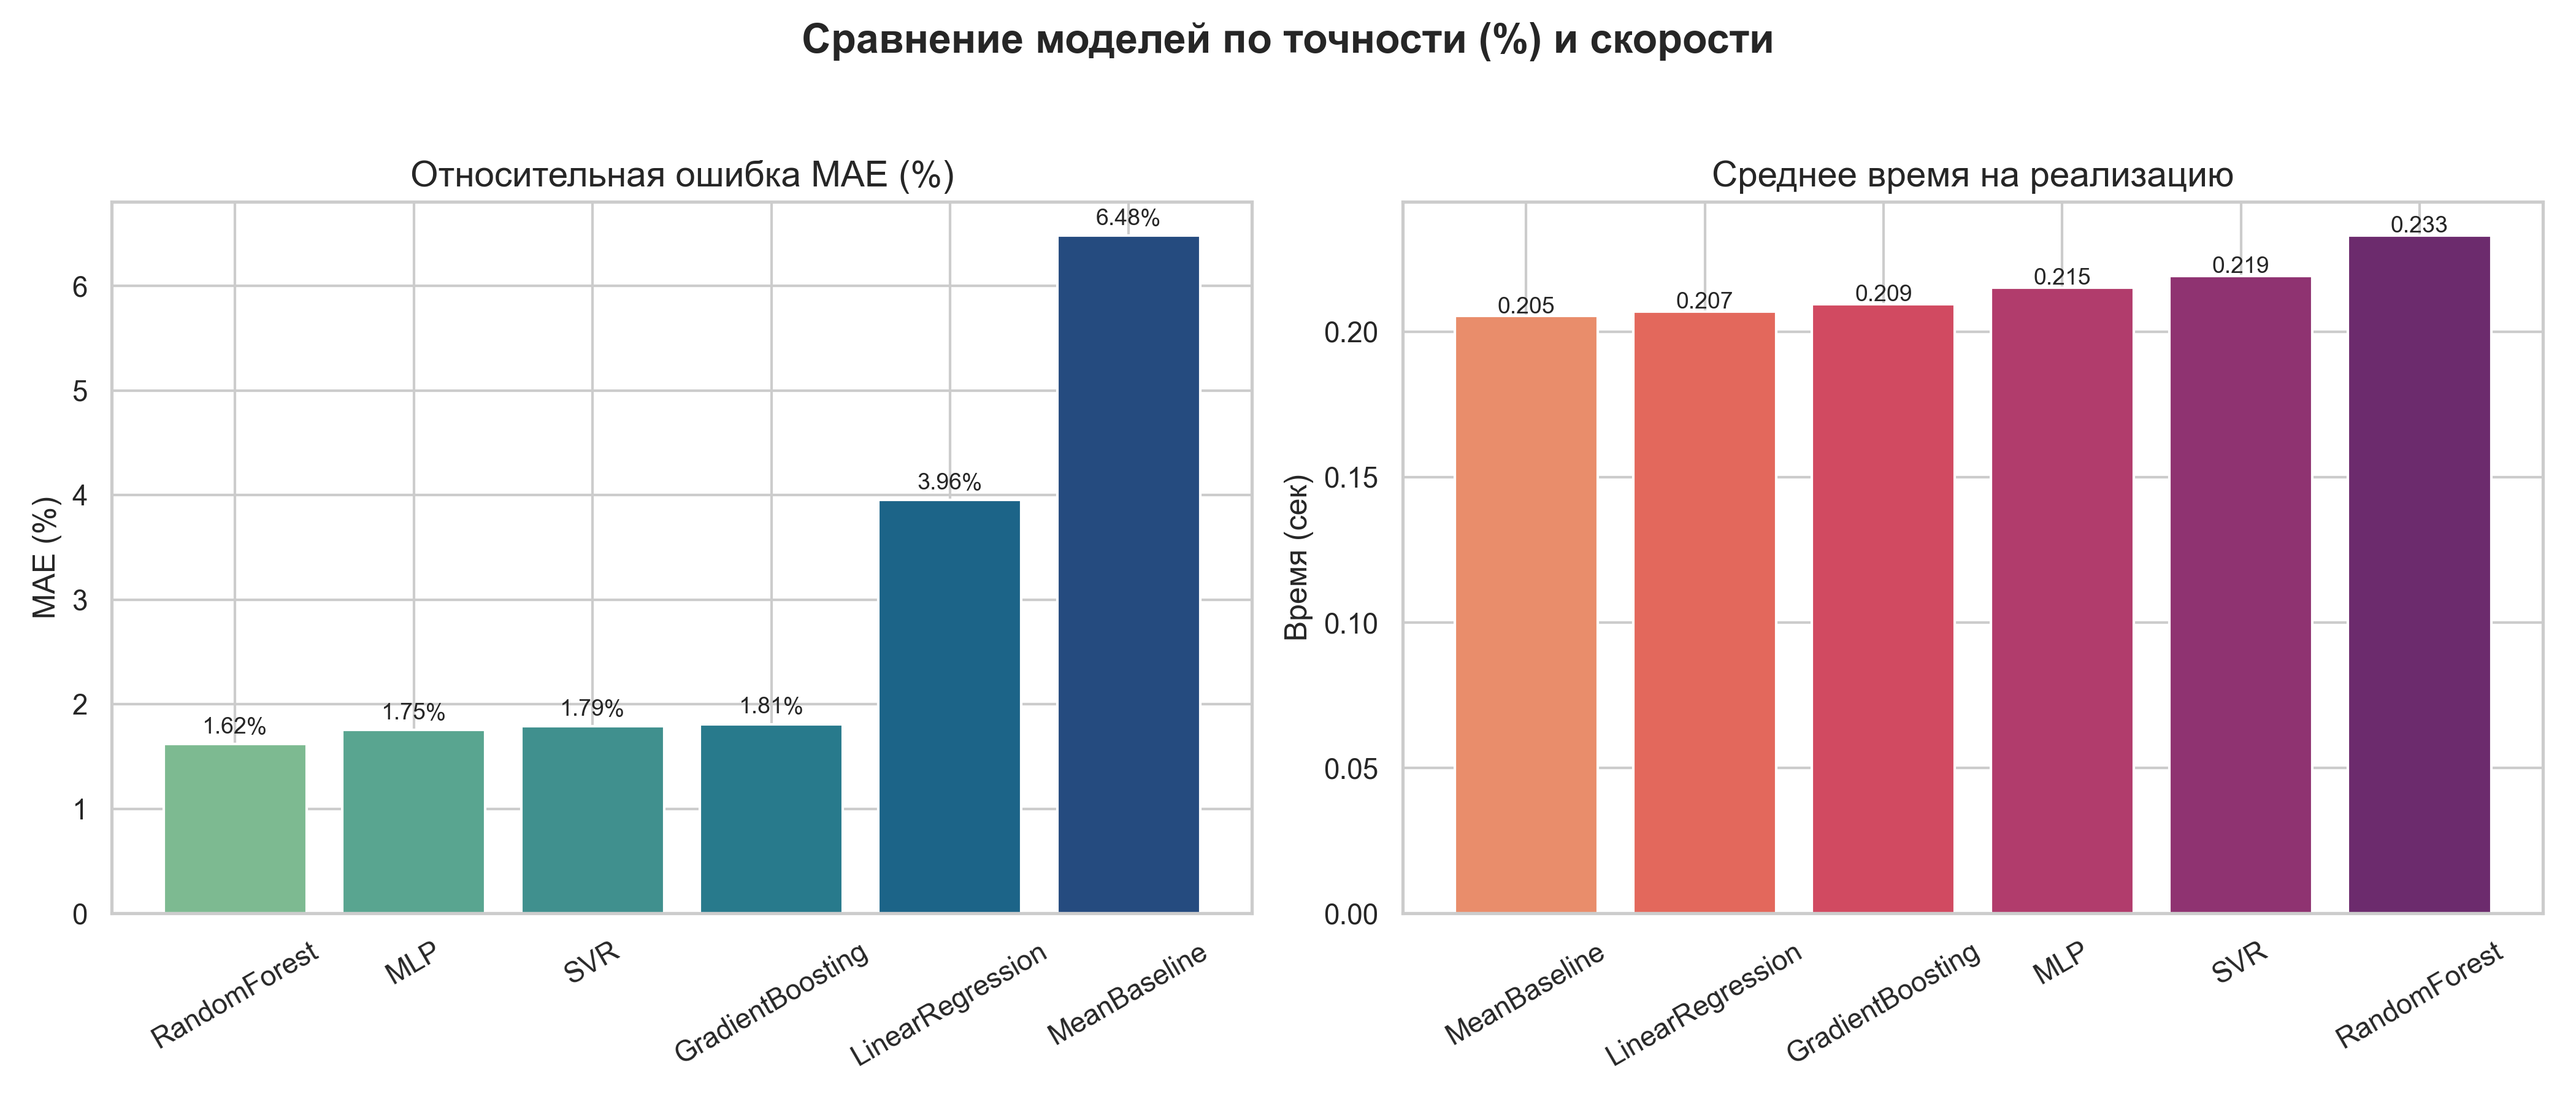
\includegraphics[width=0.85\textwidth]{/Users/macbookmike_1/PycharmProjects/PythonProject/regression/models_test/Models_test.png}
\end{center}

MeanBaseline здесь это метод, который просто берет средние значения гиперпараметров из обучающей выборки, то есть без применения машинного обучения.
Такой подход показывает наихудший результат по точности.
На рисунке видно, что остальные модели, использующие ML, показывают примерно одинаковые результаты по точности и времени работы.
В качестве итоговой модели был выбран градиентный бустинг - классическая ансамблевая модель, имеющая понятный принцип работы в отличие
от сложных нейросетевых моделей по типу MLP.

\section*{Результаты работы алгоритма}

\begin{center}
    \begin{minipage}{0.48\textwidth}
        \includegraphics[width=\linewidth]{intervals_2}
    \end{minipage}
    \hfill
    \begin{minipage}{0.48\textwidth}
        \includegraphics[width=\linewidth]{intervals_1}
    \end{minipage}
\end{center}

Видно, что алгоритм исправно работает и для случаев когда число изолированных участков не равно 3.

\section*{Алгоритм второй подзадачи}

Для повышения устойчивости и исключения нефизичных случаев проведем регуляризацию задачи (1).
\[
\text{Pe}_1 - \text{задано},\quad \text{Pe}_2 = \text{Pe}_1 - \Delta_1,\quad \text{Pe}_3 = \text{Pe}_2 - \Delta_2,\ \ldots
\]

То есть оптимизируются не сами значения $\text{Pe}_i$, а их разности $\Delta_i$, с условием $\text{Pe}_i \geq \text{Pe}_{i+1} \geq 0$.

\section*{Оценка точности}

В качестве невязки решения будем использовать удельную площадь отклонения профилей утечек:
В качестве невязки решения будем использовать удельную площадь отклонения профилей утечек:
В качестве невязки решения будем использовать удельную площадь отклонения профилей утечек:
\[
J = \sqrt{ \frac{1}{z_{\text{max}} - z_{\text{min}}} \int_{z_{\text{min}}}^{z_{\text{max}}} \left| Q(z) - \hat{Q}(z) \right|^2 dz } \tag{4}
\]

\section*{Численный метод оптимизации}
По умолчанию во всех примерах используется классический для решения задач о наименьших квадратов метод Левенберга-Марквардта, не требующий задания якобиана
функционала (1) и хорошо сходящийся даже при плохом начальном приближении.

\section*{Результаты оптимизации}

\begin{center}
    \begin{minipage}{0.48\textwidth}
        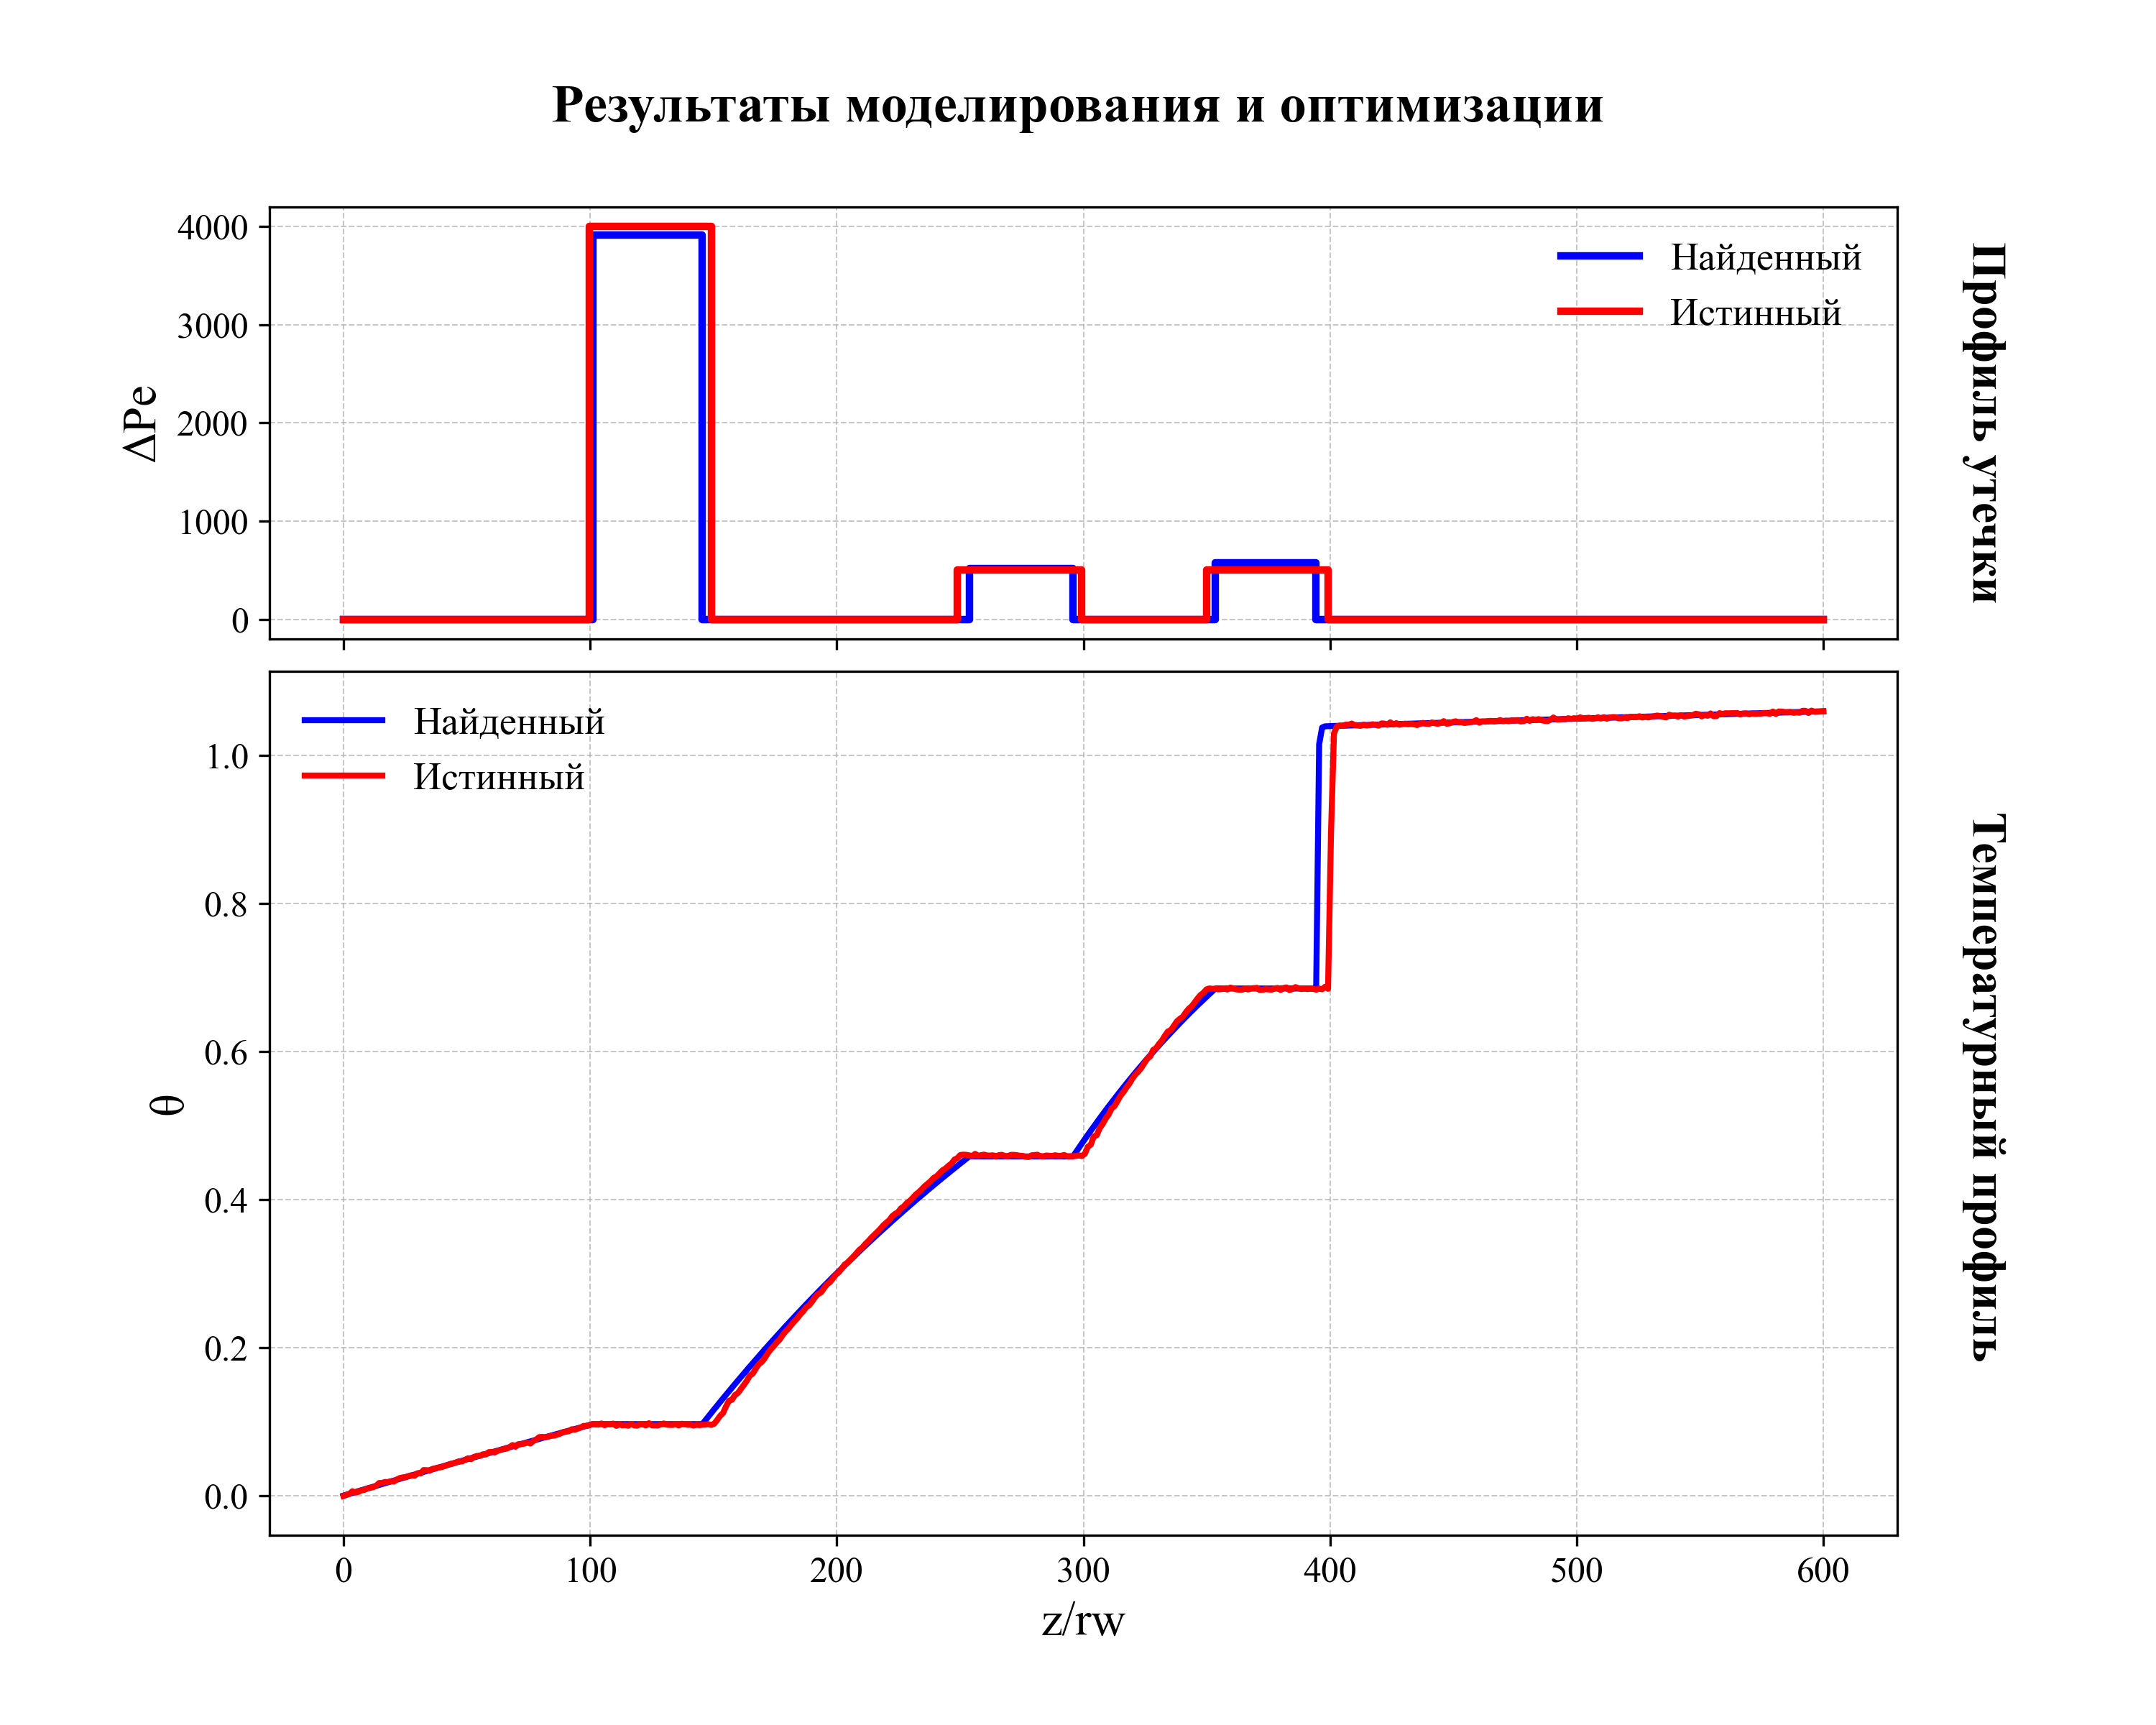
\includegraphics[width=\linewidth]{/Users/macbookmike_1/PycharmProjects/PythonProject/test_samle/Профиль утечки}
    \end{minipage}
    \hfill
    \begin{minipage}{0.48\textwidth}
        \includegraphics[width=\linewidth]{/Users/macbookmike_1/Downloads/optimization_path}
    \end{minipage}
\end{center}

\begin{center}
    \begin{minipage}{0.48\textwidth}
        \includegraphics[width=\linewidth]{/Users/macbookmike_1/Downloads/residuals_animation}
    \end{minipage}
    \hfill
    \begin{minipage}{0.48\textwidth}
        \includegraphics[width=\linewidth]{/Users/macbookmike_1/Downloads/pe_animation}
    \end{minipage}
\end{center}

\section*{Сравнение разных методов оптимизации}

\begin{center}
    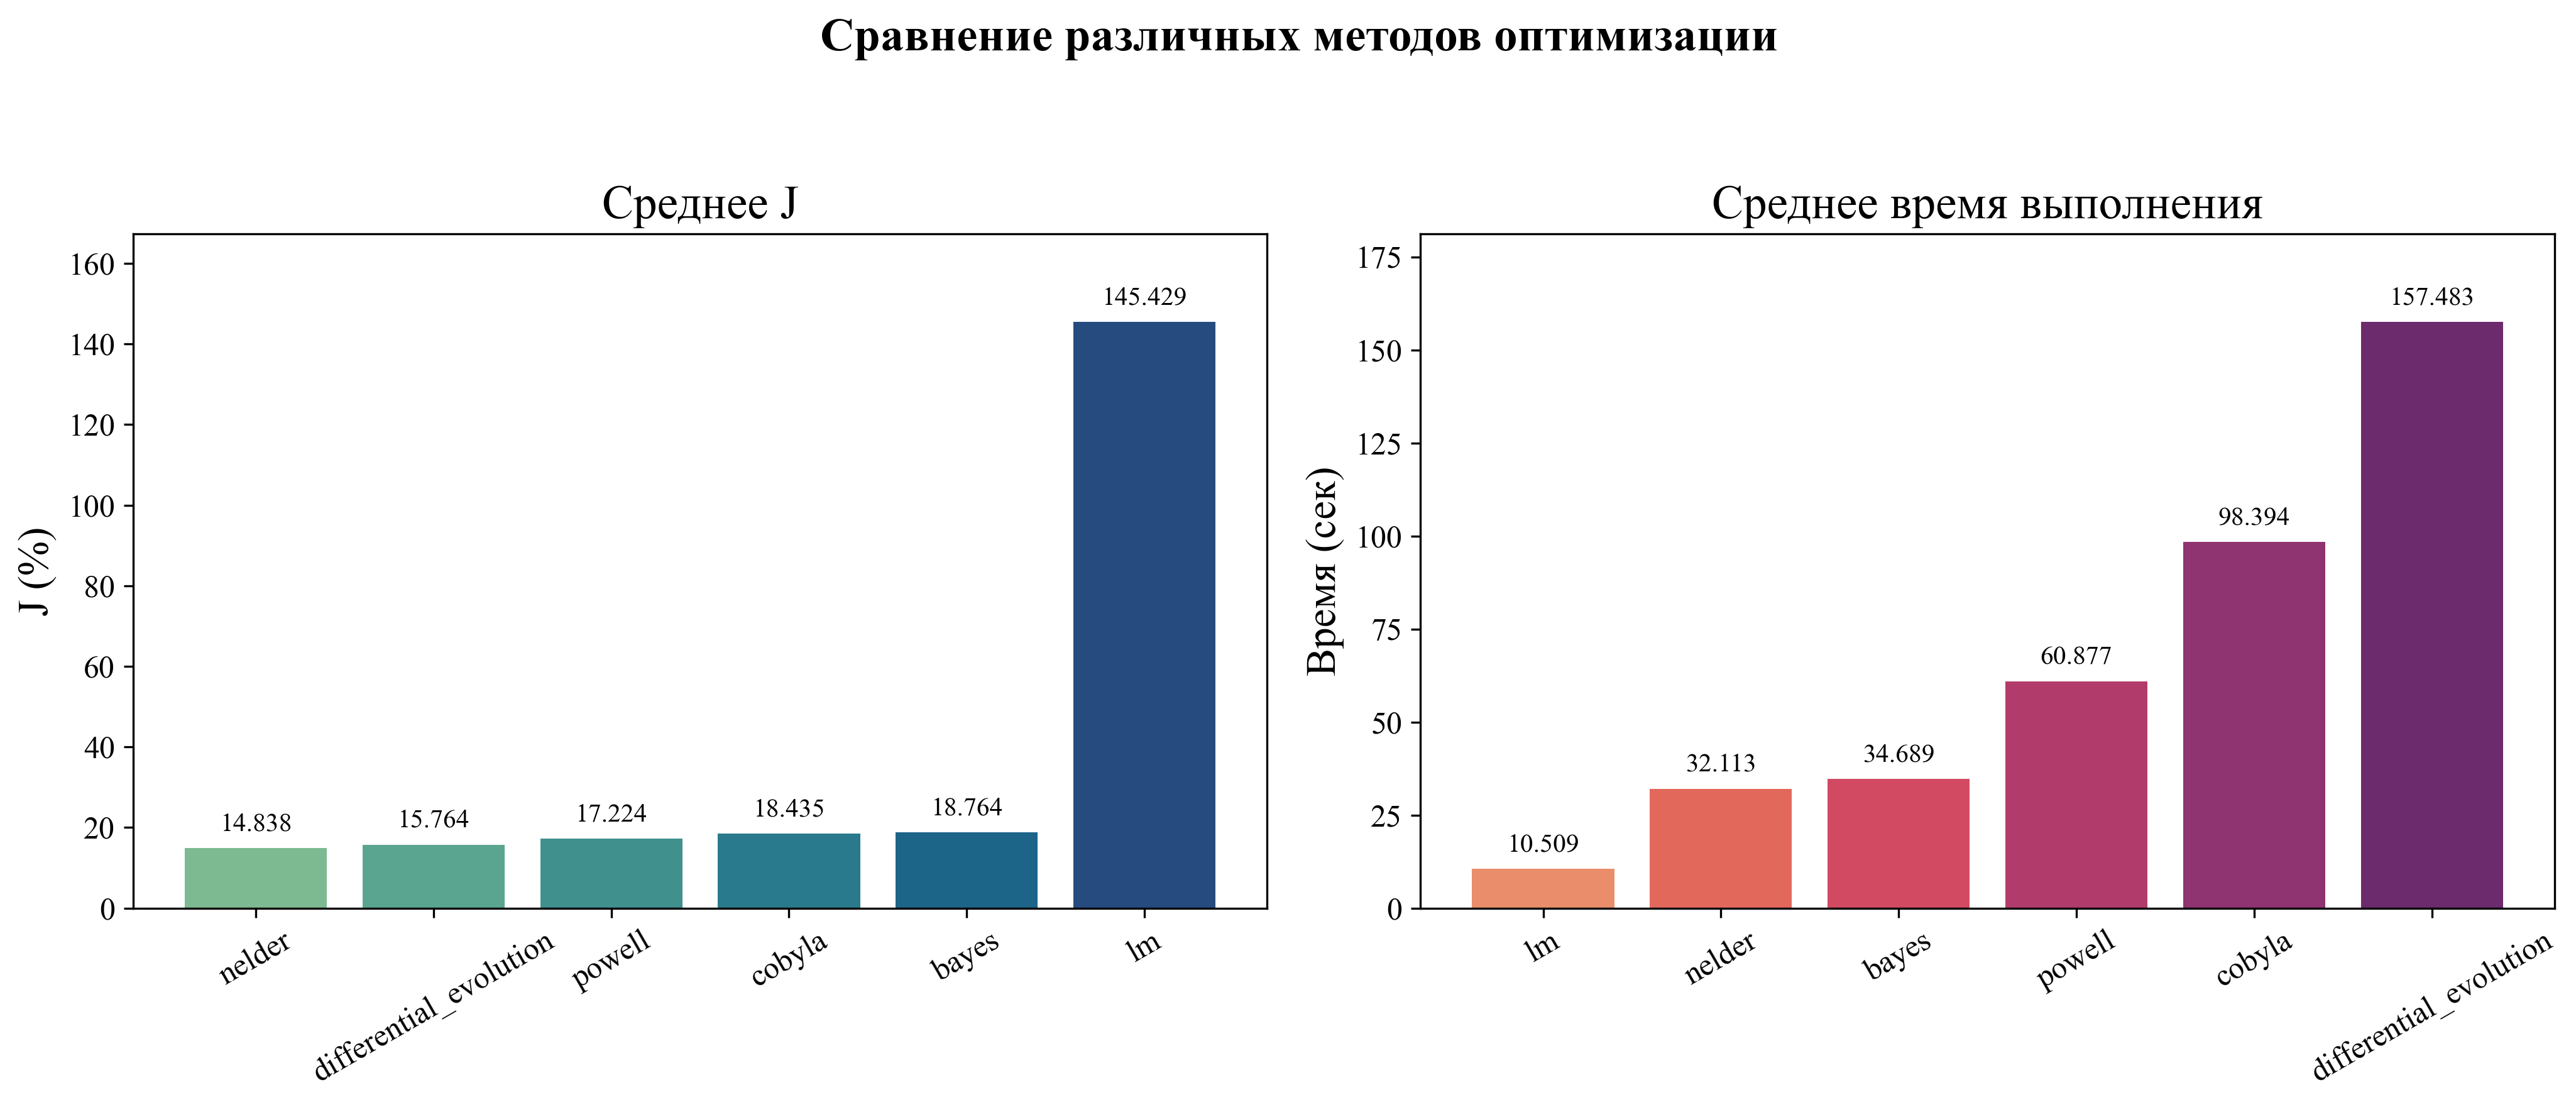
\includegraphics[width=0.85\textwidth]{/Users/macbookmike_1/PycharmProjects/PythonProject/stability_tests/data/charts/stability_optimaizers/barplot_graph}
\end{center}

На графике видны подозрительно сильные отличия между методами: метод Левенберга имеет среднее значение невязки почти в 2 раза
большее чем методы Нельдера и Пауэла, хоть и работает быстрее. Надо будет пересчитать, задавая для каждого метода одинаковую генерацию шума.

\section*{Устойчивость и чувствительность общего алгоритма}

Необходимо удостовериться в ограниченности отклонения приближённого (квази) решения при наличии ограниченной погрешности
исходных данных: для каждого $\delta > 0$ генерировать $N$ реализаций шума $\{\xi_i\}_{i=1}^N$, $\|\xi_i\| \leq \delta$,
для каждой реализации решать задачу с получением своей интегральной метрики отклонения (4),
для этой случайной величины произвести статистическую оценку — математическое
ожидание $\mathbb{E}\rho$ и дисперсию $\mathrm{D}\rho$. Построить зависимость $\mathbb{E}\rho(\delta)$ и $\mathrm{D}\rho(\delta)$.

\section*{Результаты расчетов}
Во всех тестах использовался пример профиля температуры, содержащий 4 изолированных интервала. Параметры задачи: A = 5, Pe = [5000, 2000, 1000, 0]

\begin{center}
    \begin{minipage}{0.48\textwidth}
        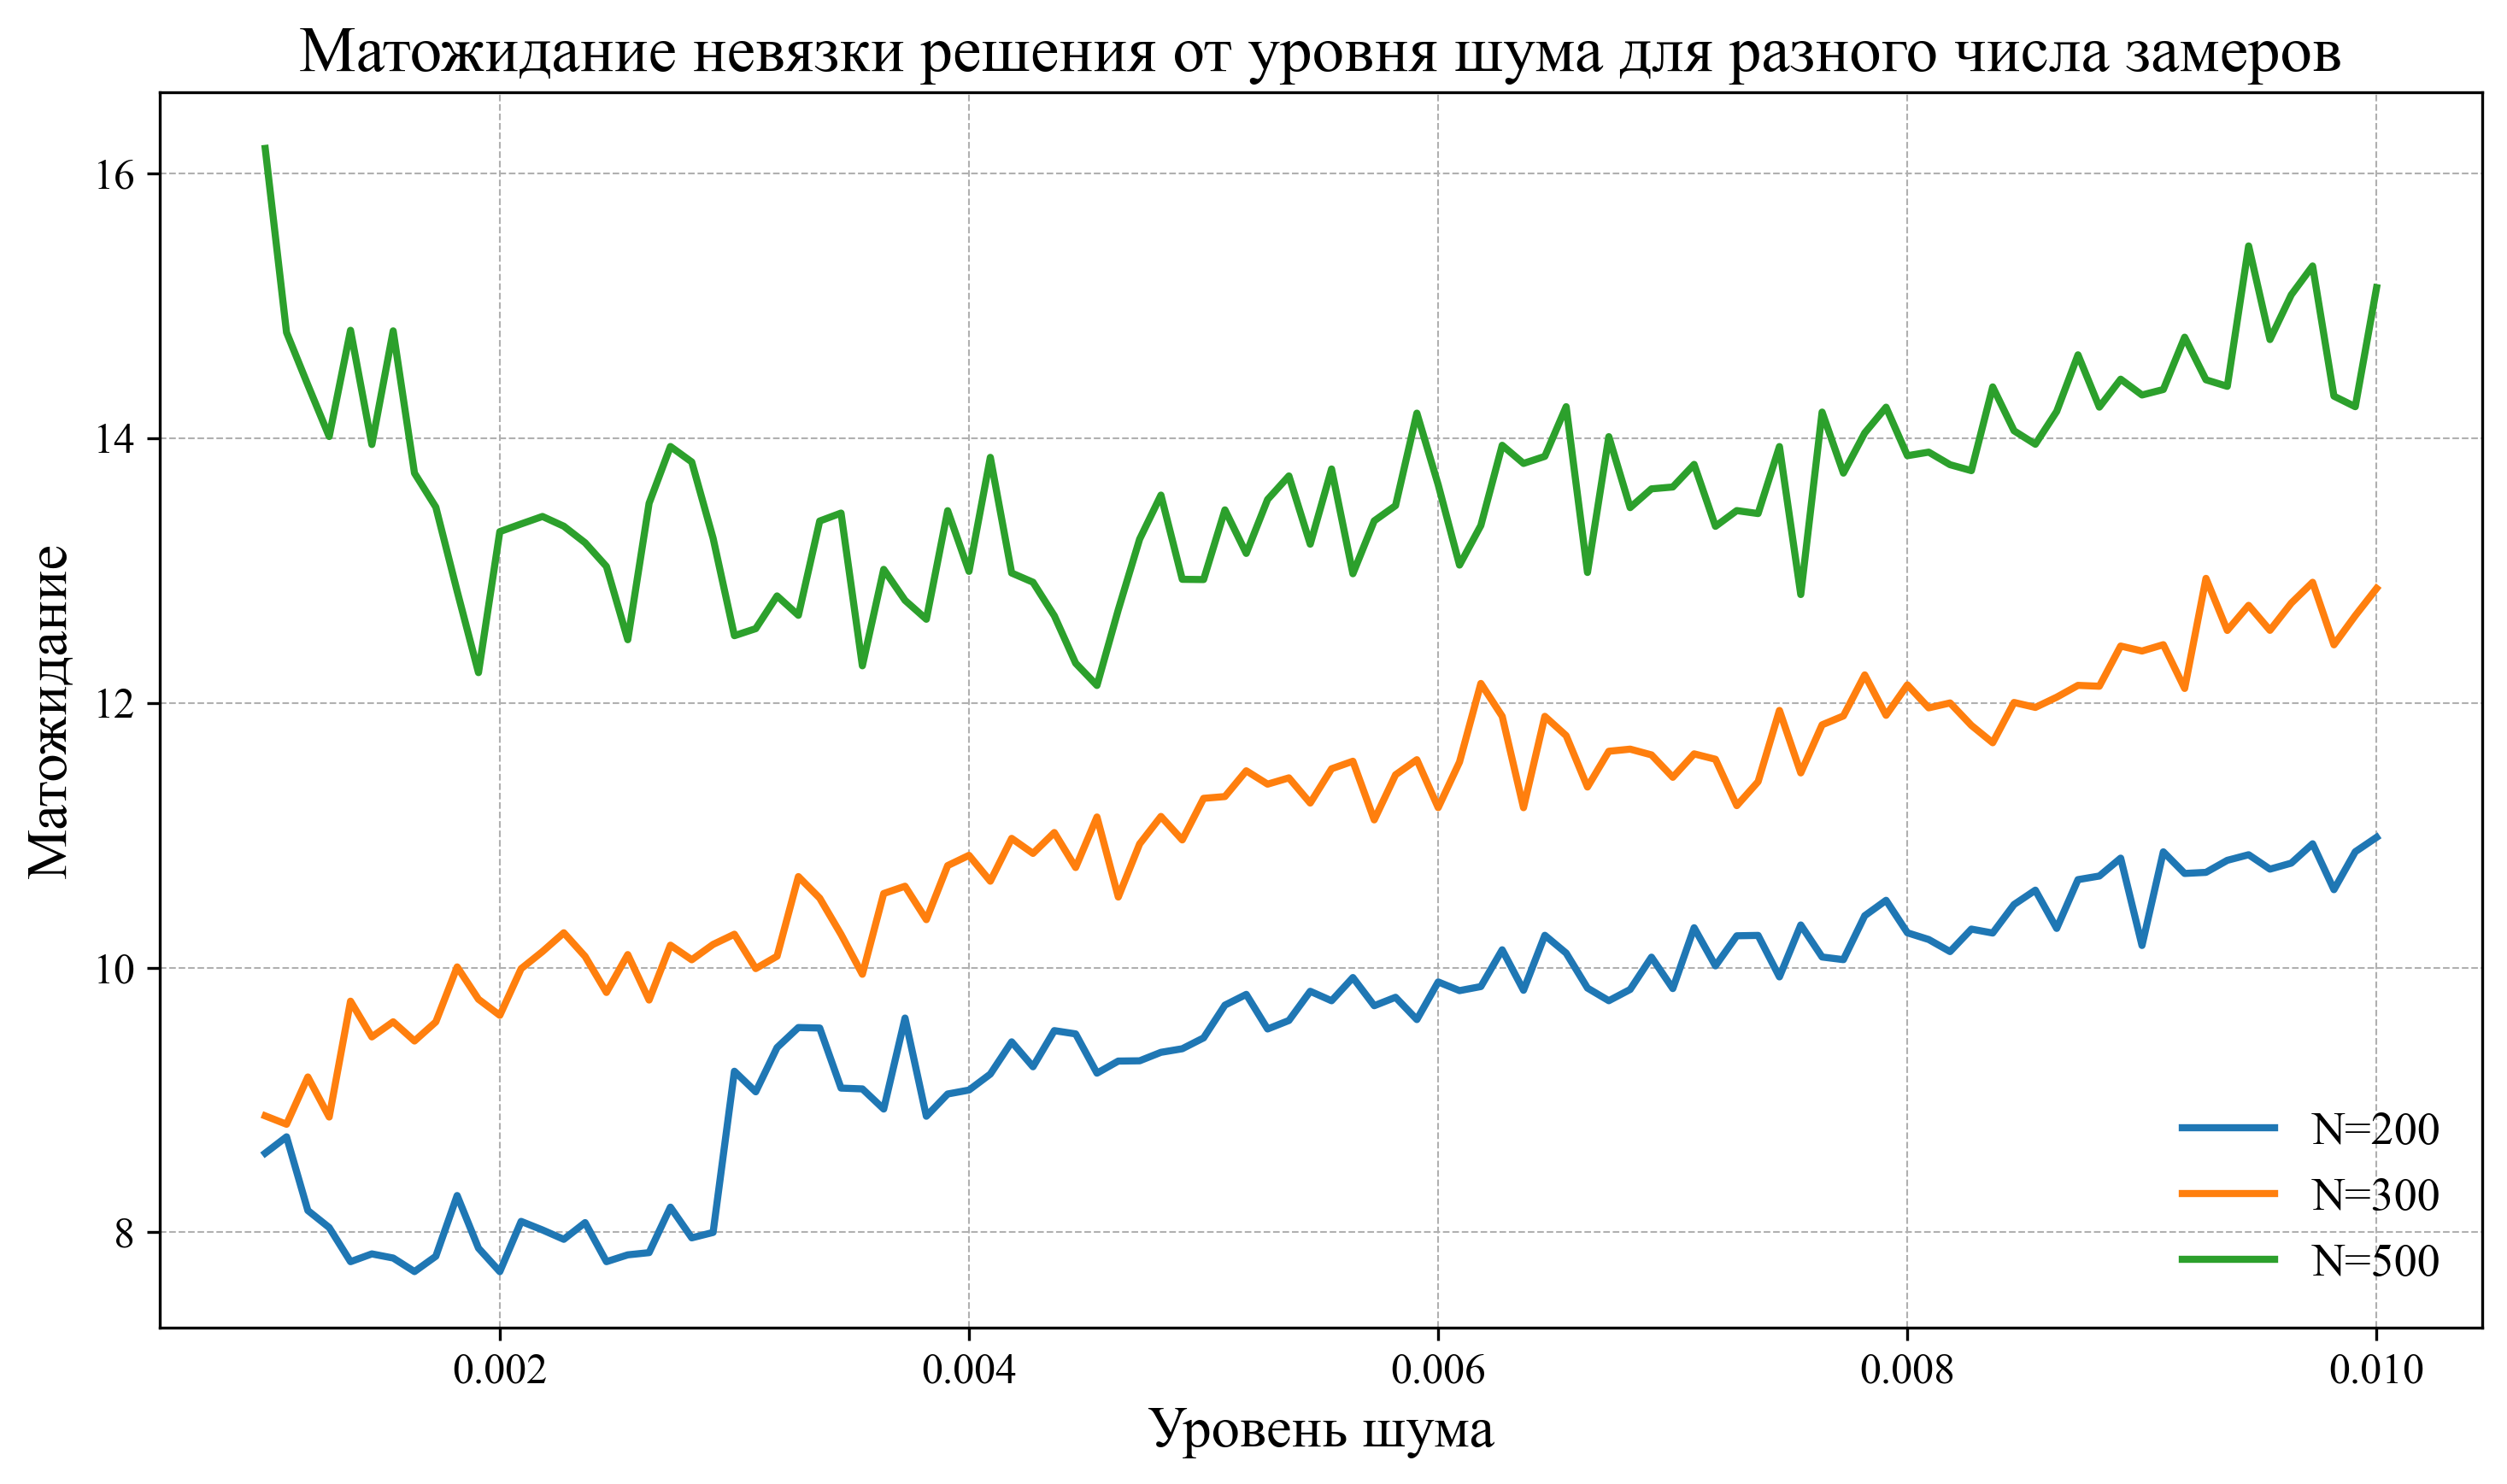
\includegraphics[width=\linewidth]{/Users/macbookmike_1/PycharmProjects/PythonProject/stability_tests/data/charts/stability_std_N_samples/mean_deviation.png}
    \end{minipage}
    \hfill
    \begin{minipage}{0.48\textwidth}
        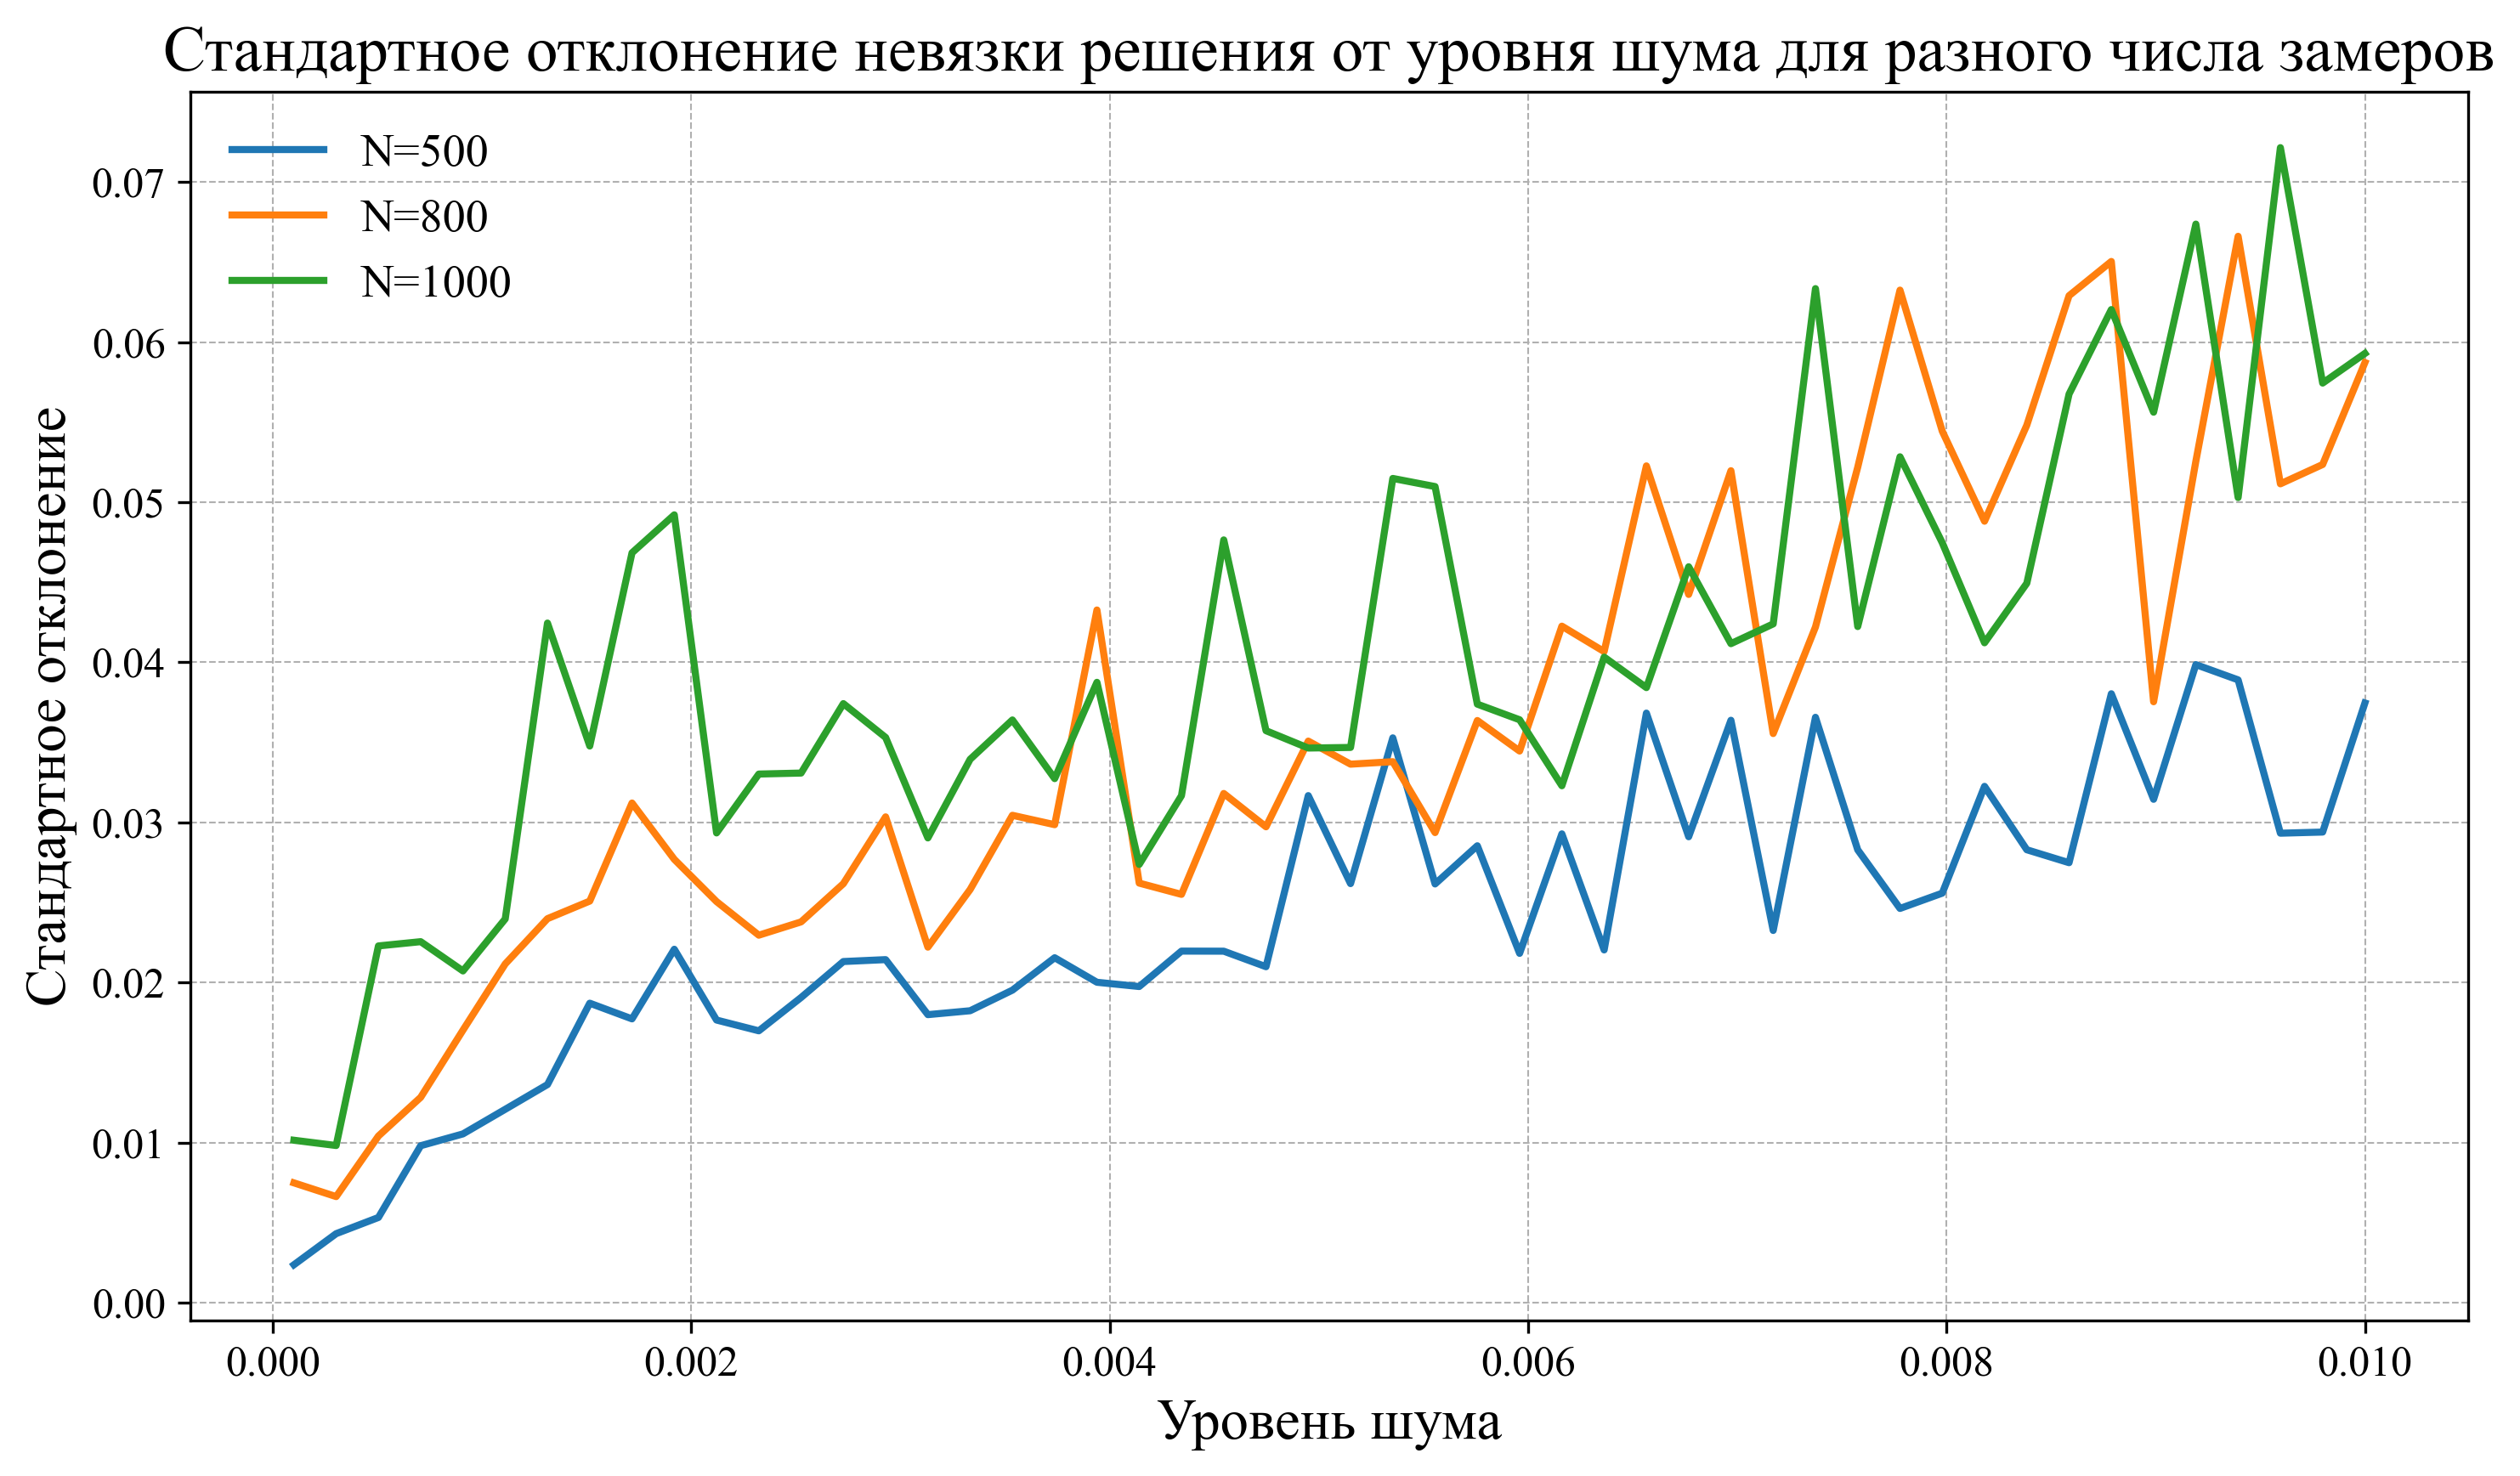
\includegraphics[width=\linewidth]{/Users/macbookmike_1/PycharmProjects/PythonProject/stability_tests/data/charts/stability_std_N_samples/std_deviation}
    \end{minipage}
\end{center}

Видна общая ограниченность решений. Но с увеличением числа
замеров, как будто бы падает точность, что довольно контринтуитивно. На самом деле, это не совсем так. При большем числе
замеров появляется больше экстремальных значений, которые растягивают результаты, но в среднем значения метрики
меньше. Это видно на общей гистограмме.

\begin{center}
    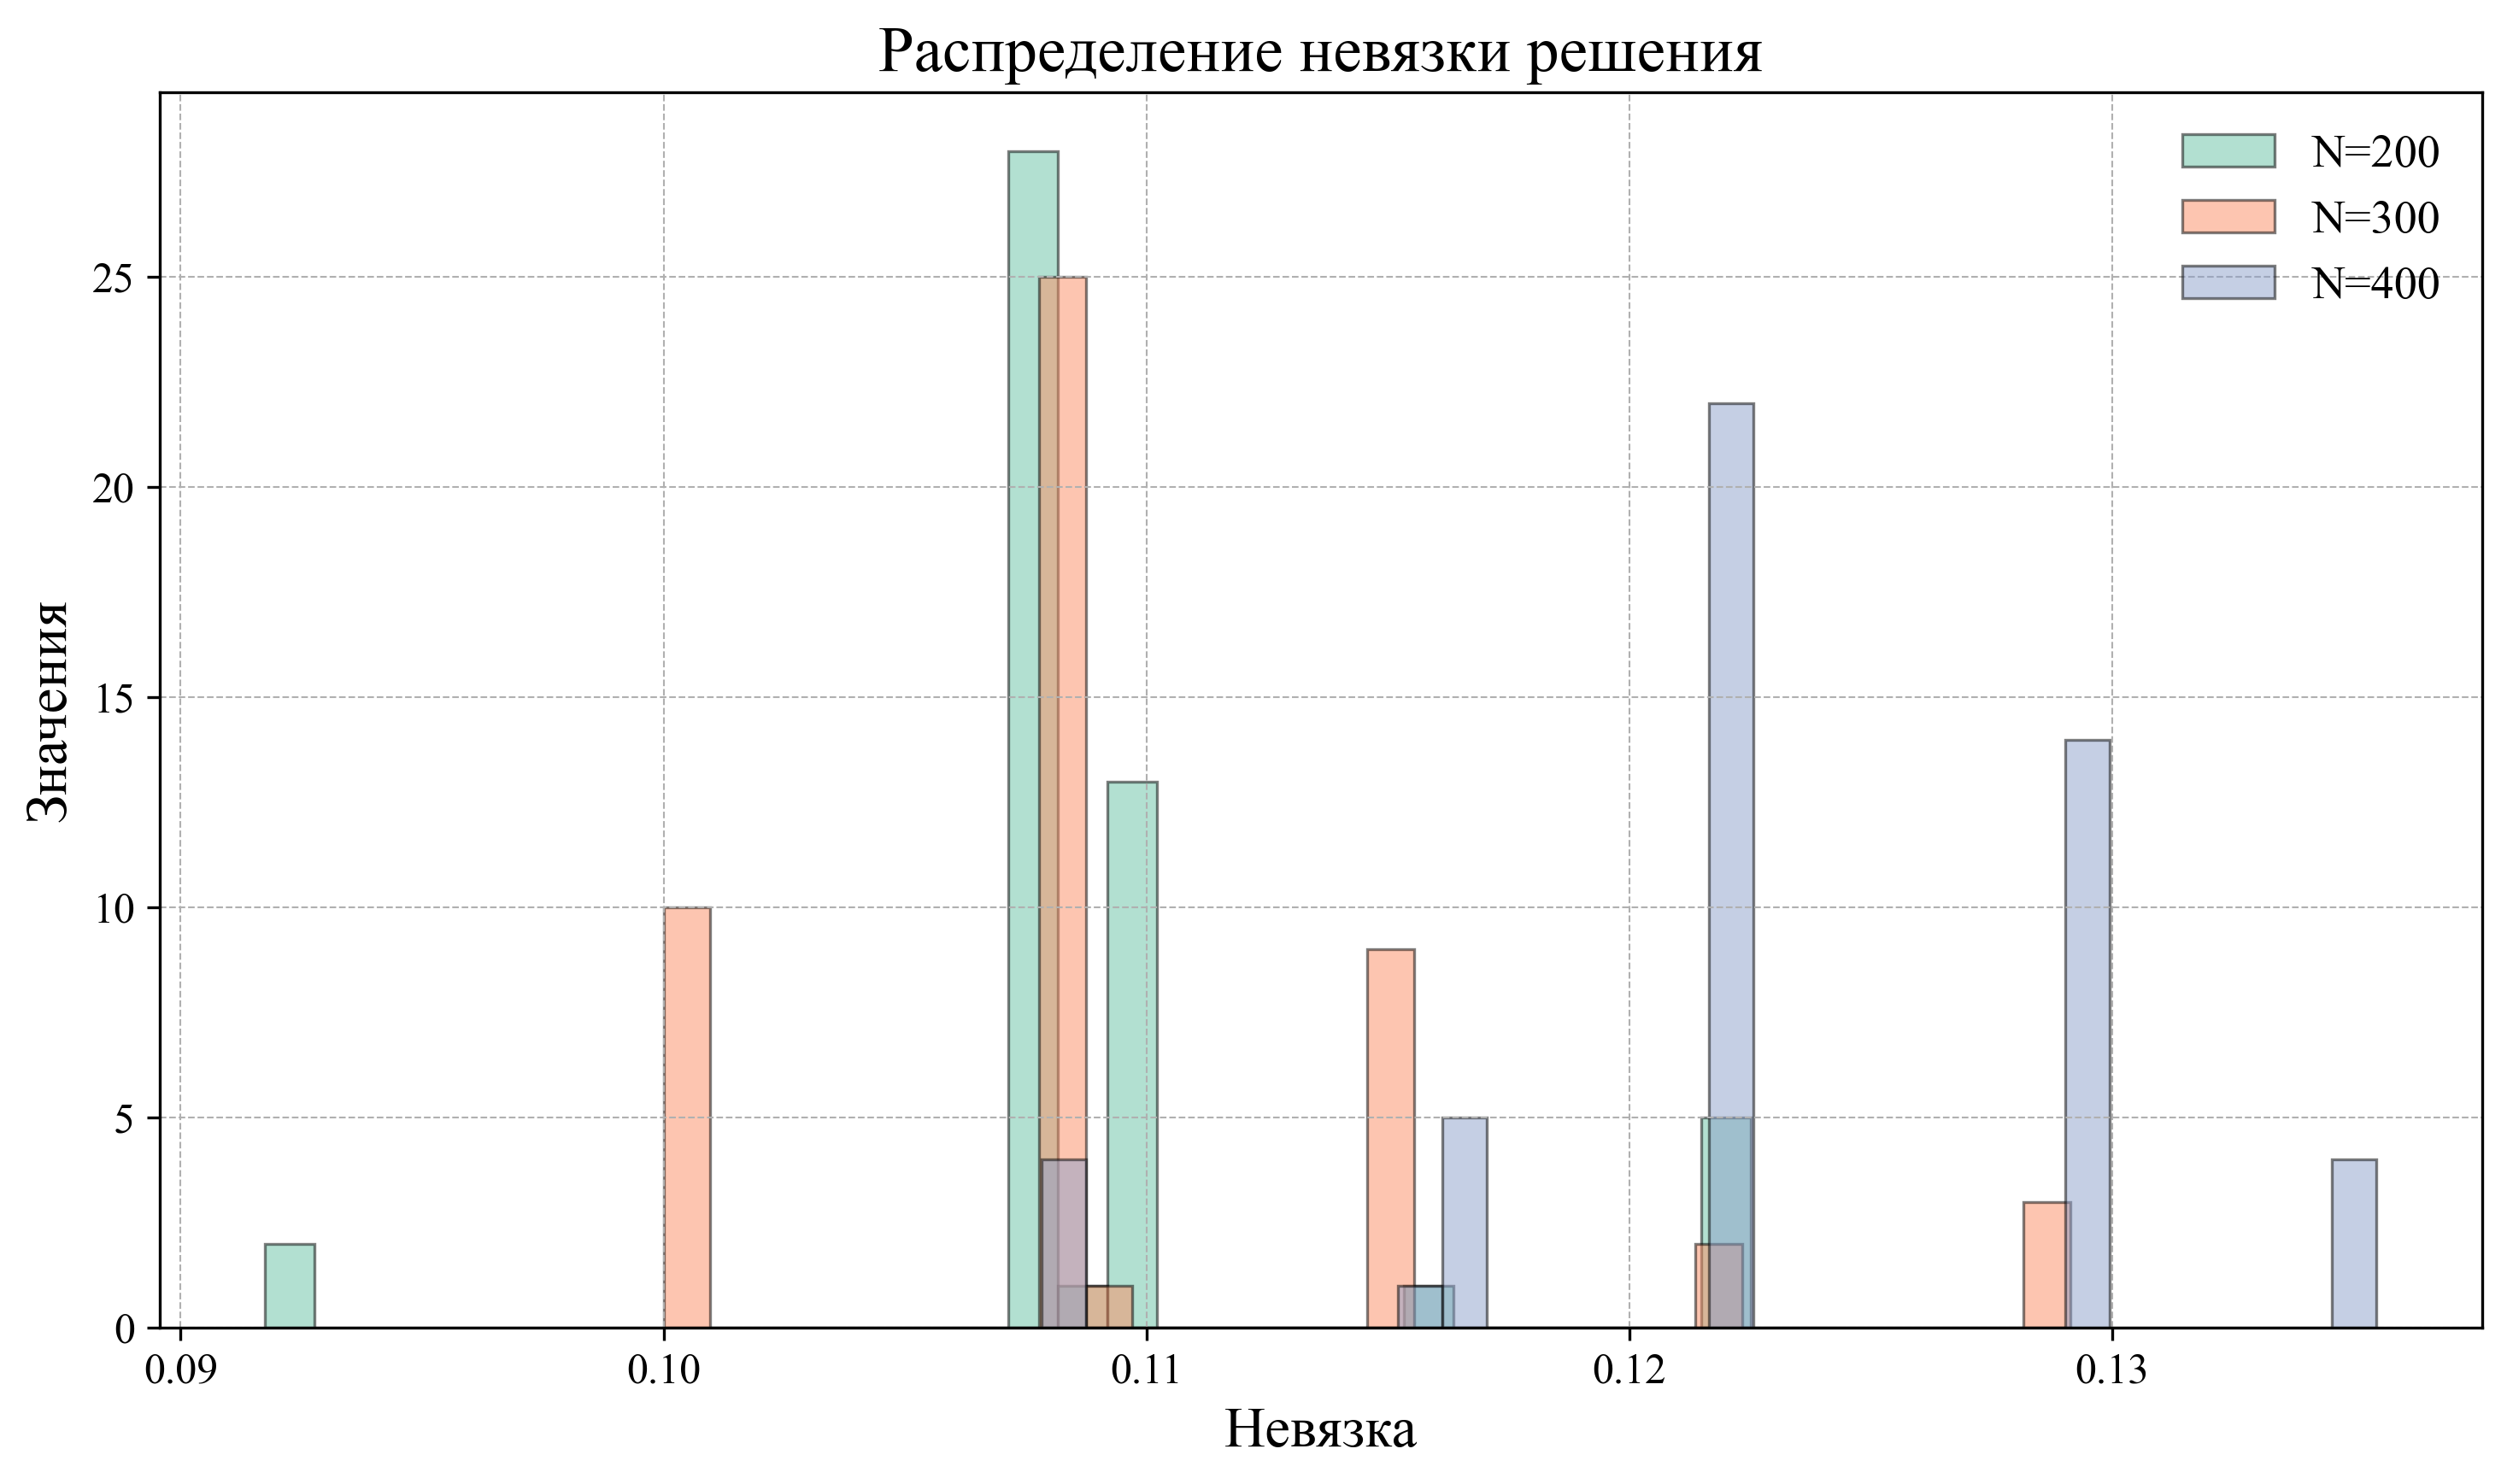
\includegraphics[width=0.85\textwidth]{/Users/macbookmike_1/PycharmProjects/PythonProject/stability_tests/data/charts/stability_std_N_samples/histogram_combined}
\end{center}

Для N = 500 заметен более тяжелый правый хвост распределения.
\vspace{0.5em}

Это связано с алгоритмом
первой подзадачи. Во-первых, модель обучалась на выборке, состоящей только из
малого количества замеров. Во-вторых, при больших значениях N, нужно увеличивать размер окна для
сглаживания, а в алгоритме пока стоит фиксированный размер. Из-за этого в результате сглаживания размываются некоторые участки кривой и растет
погрешность по границам и как следствие общая площадь отклонения. (вообще в
идеале добавить размер окна в обучающую выборку как третий гиперпараметр)


\begin{center}
    \begin{minipage}{0.48\textwidth}
        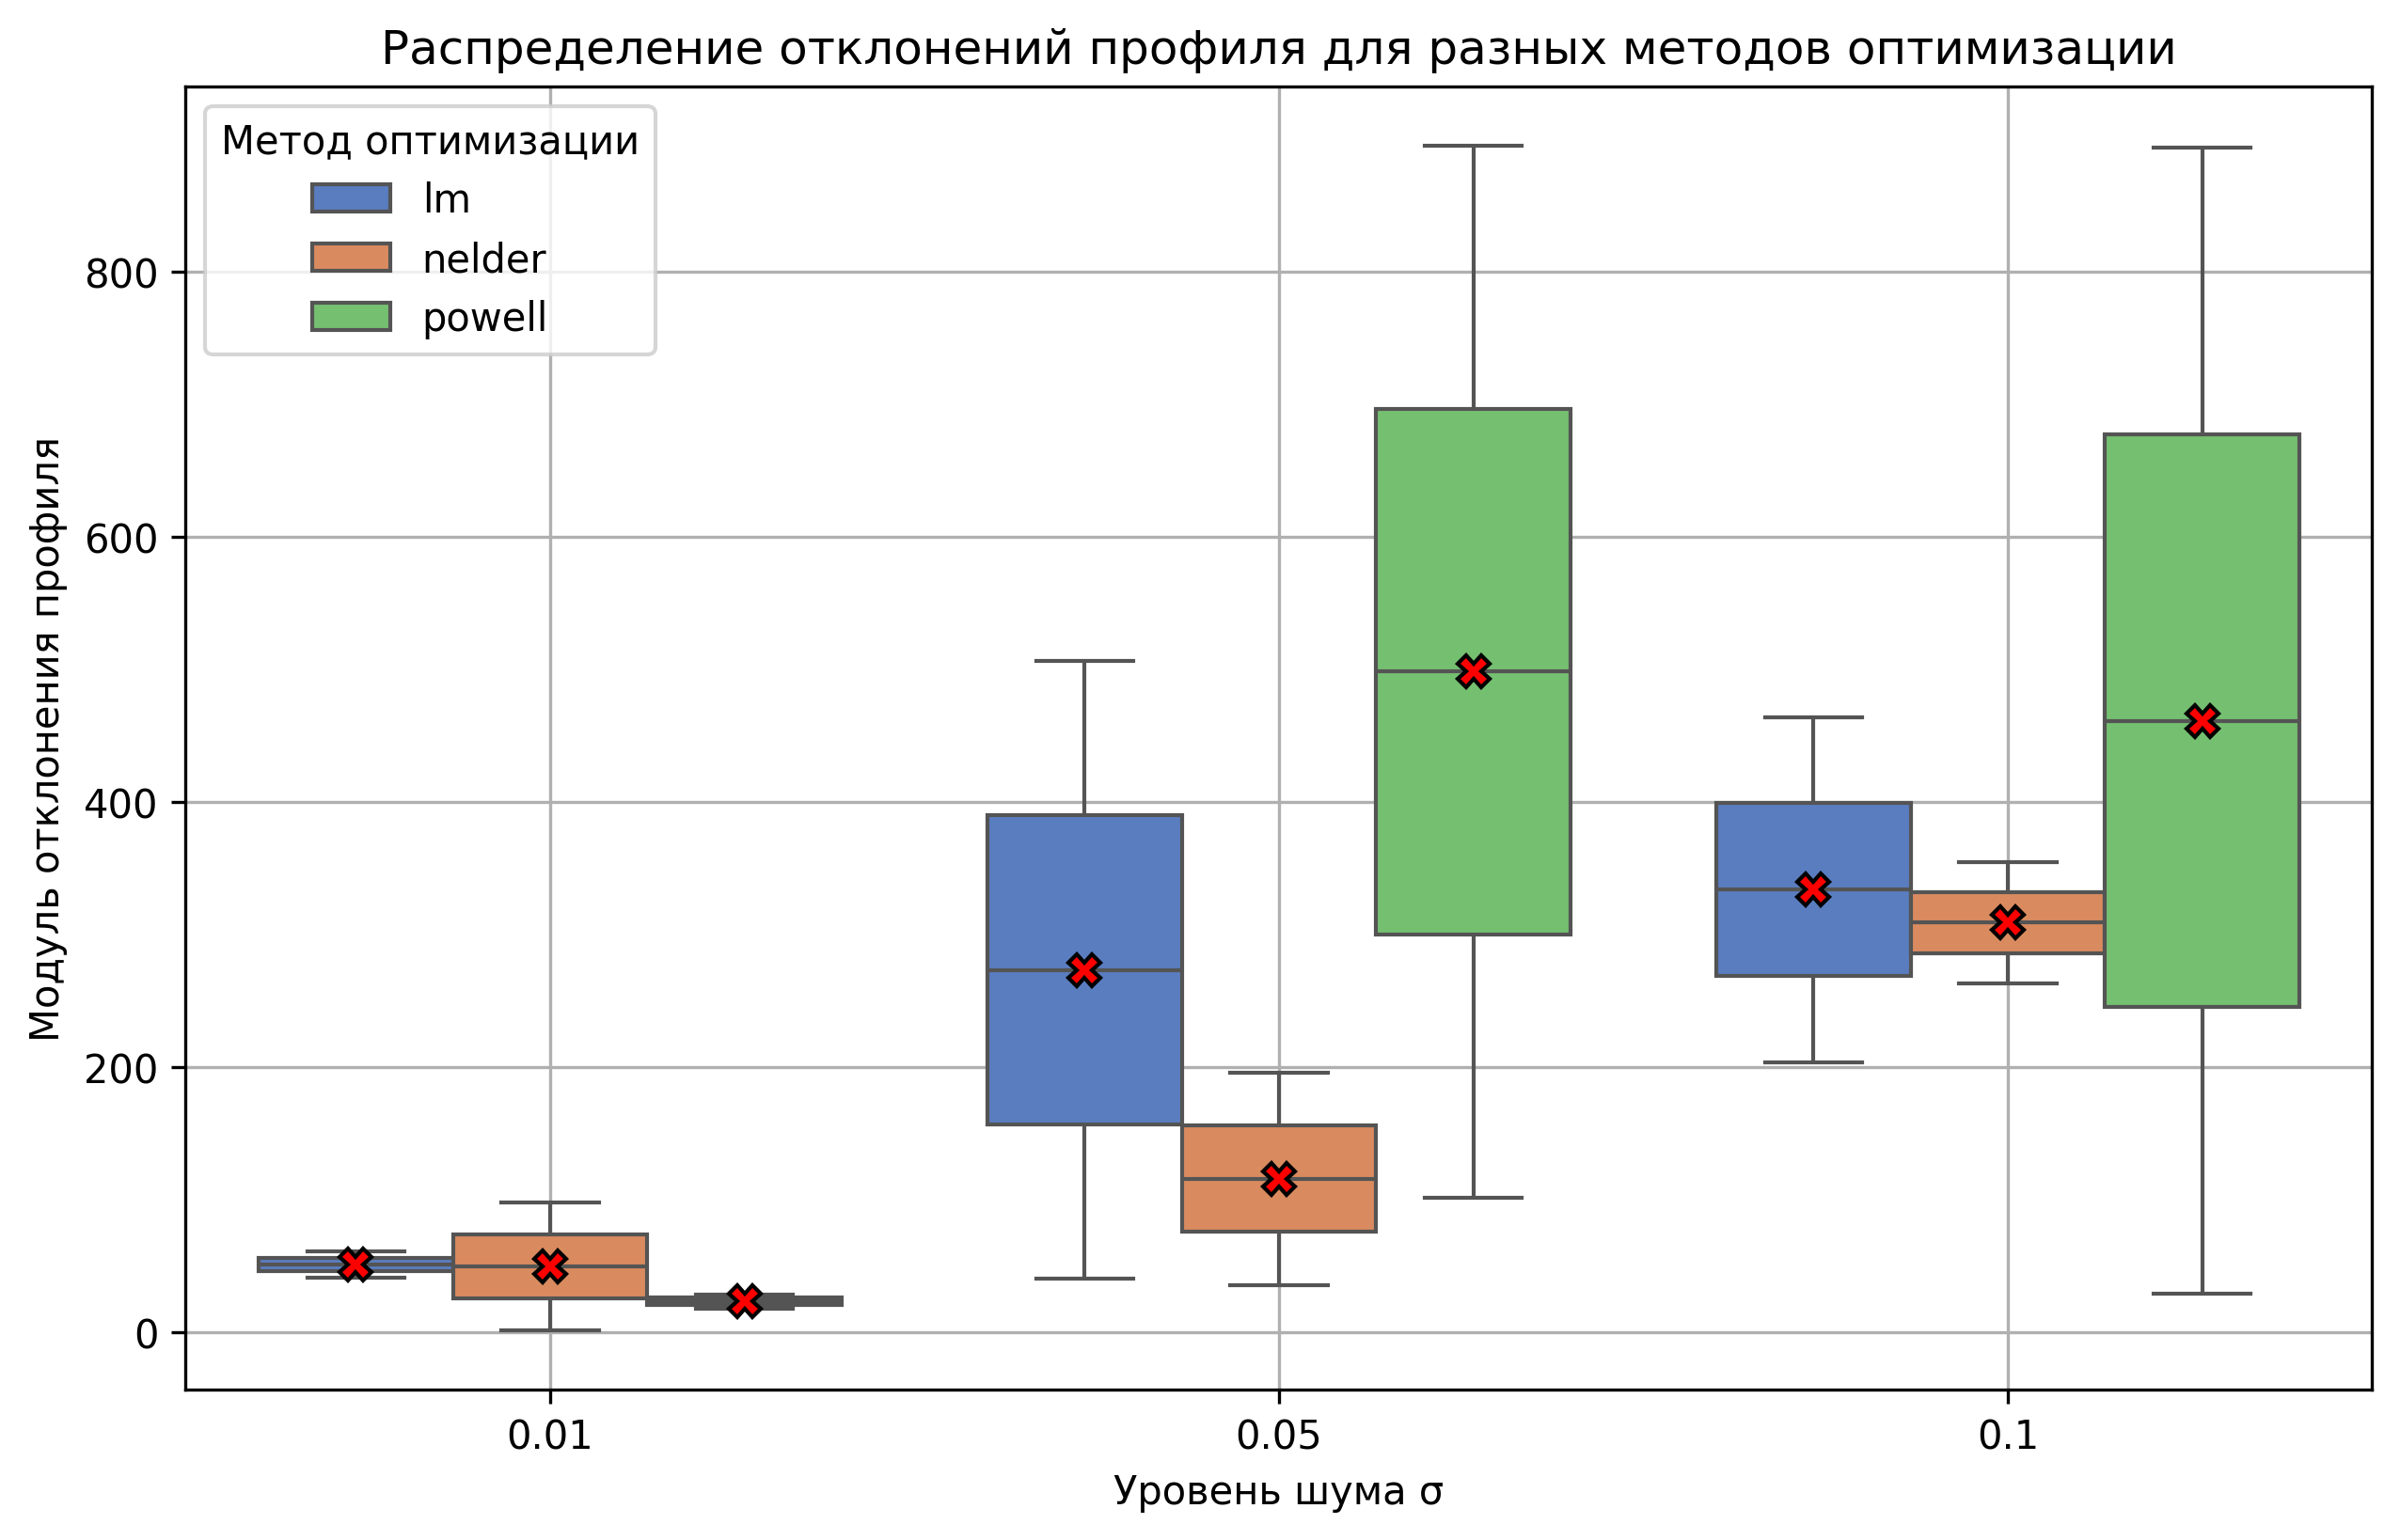
\includegraphics[width=\linewidth]{/Users/macbookmike_1/PycharmProjects/PythonProject/stability_tests/data/charts/stability_N_samples/boxplot_graph}
    \end{minipage}
    \hfill
    \begin{minipage}{0.48\textwidth}
        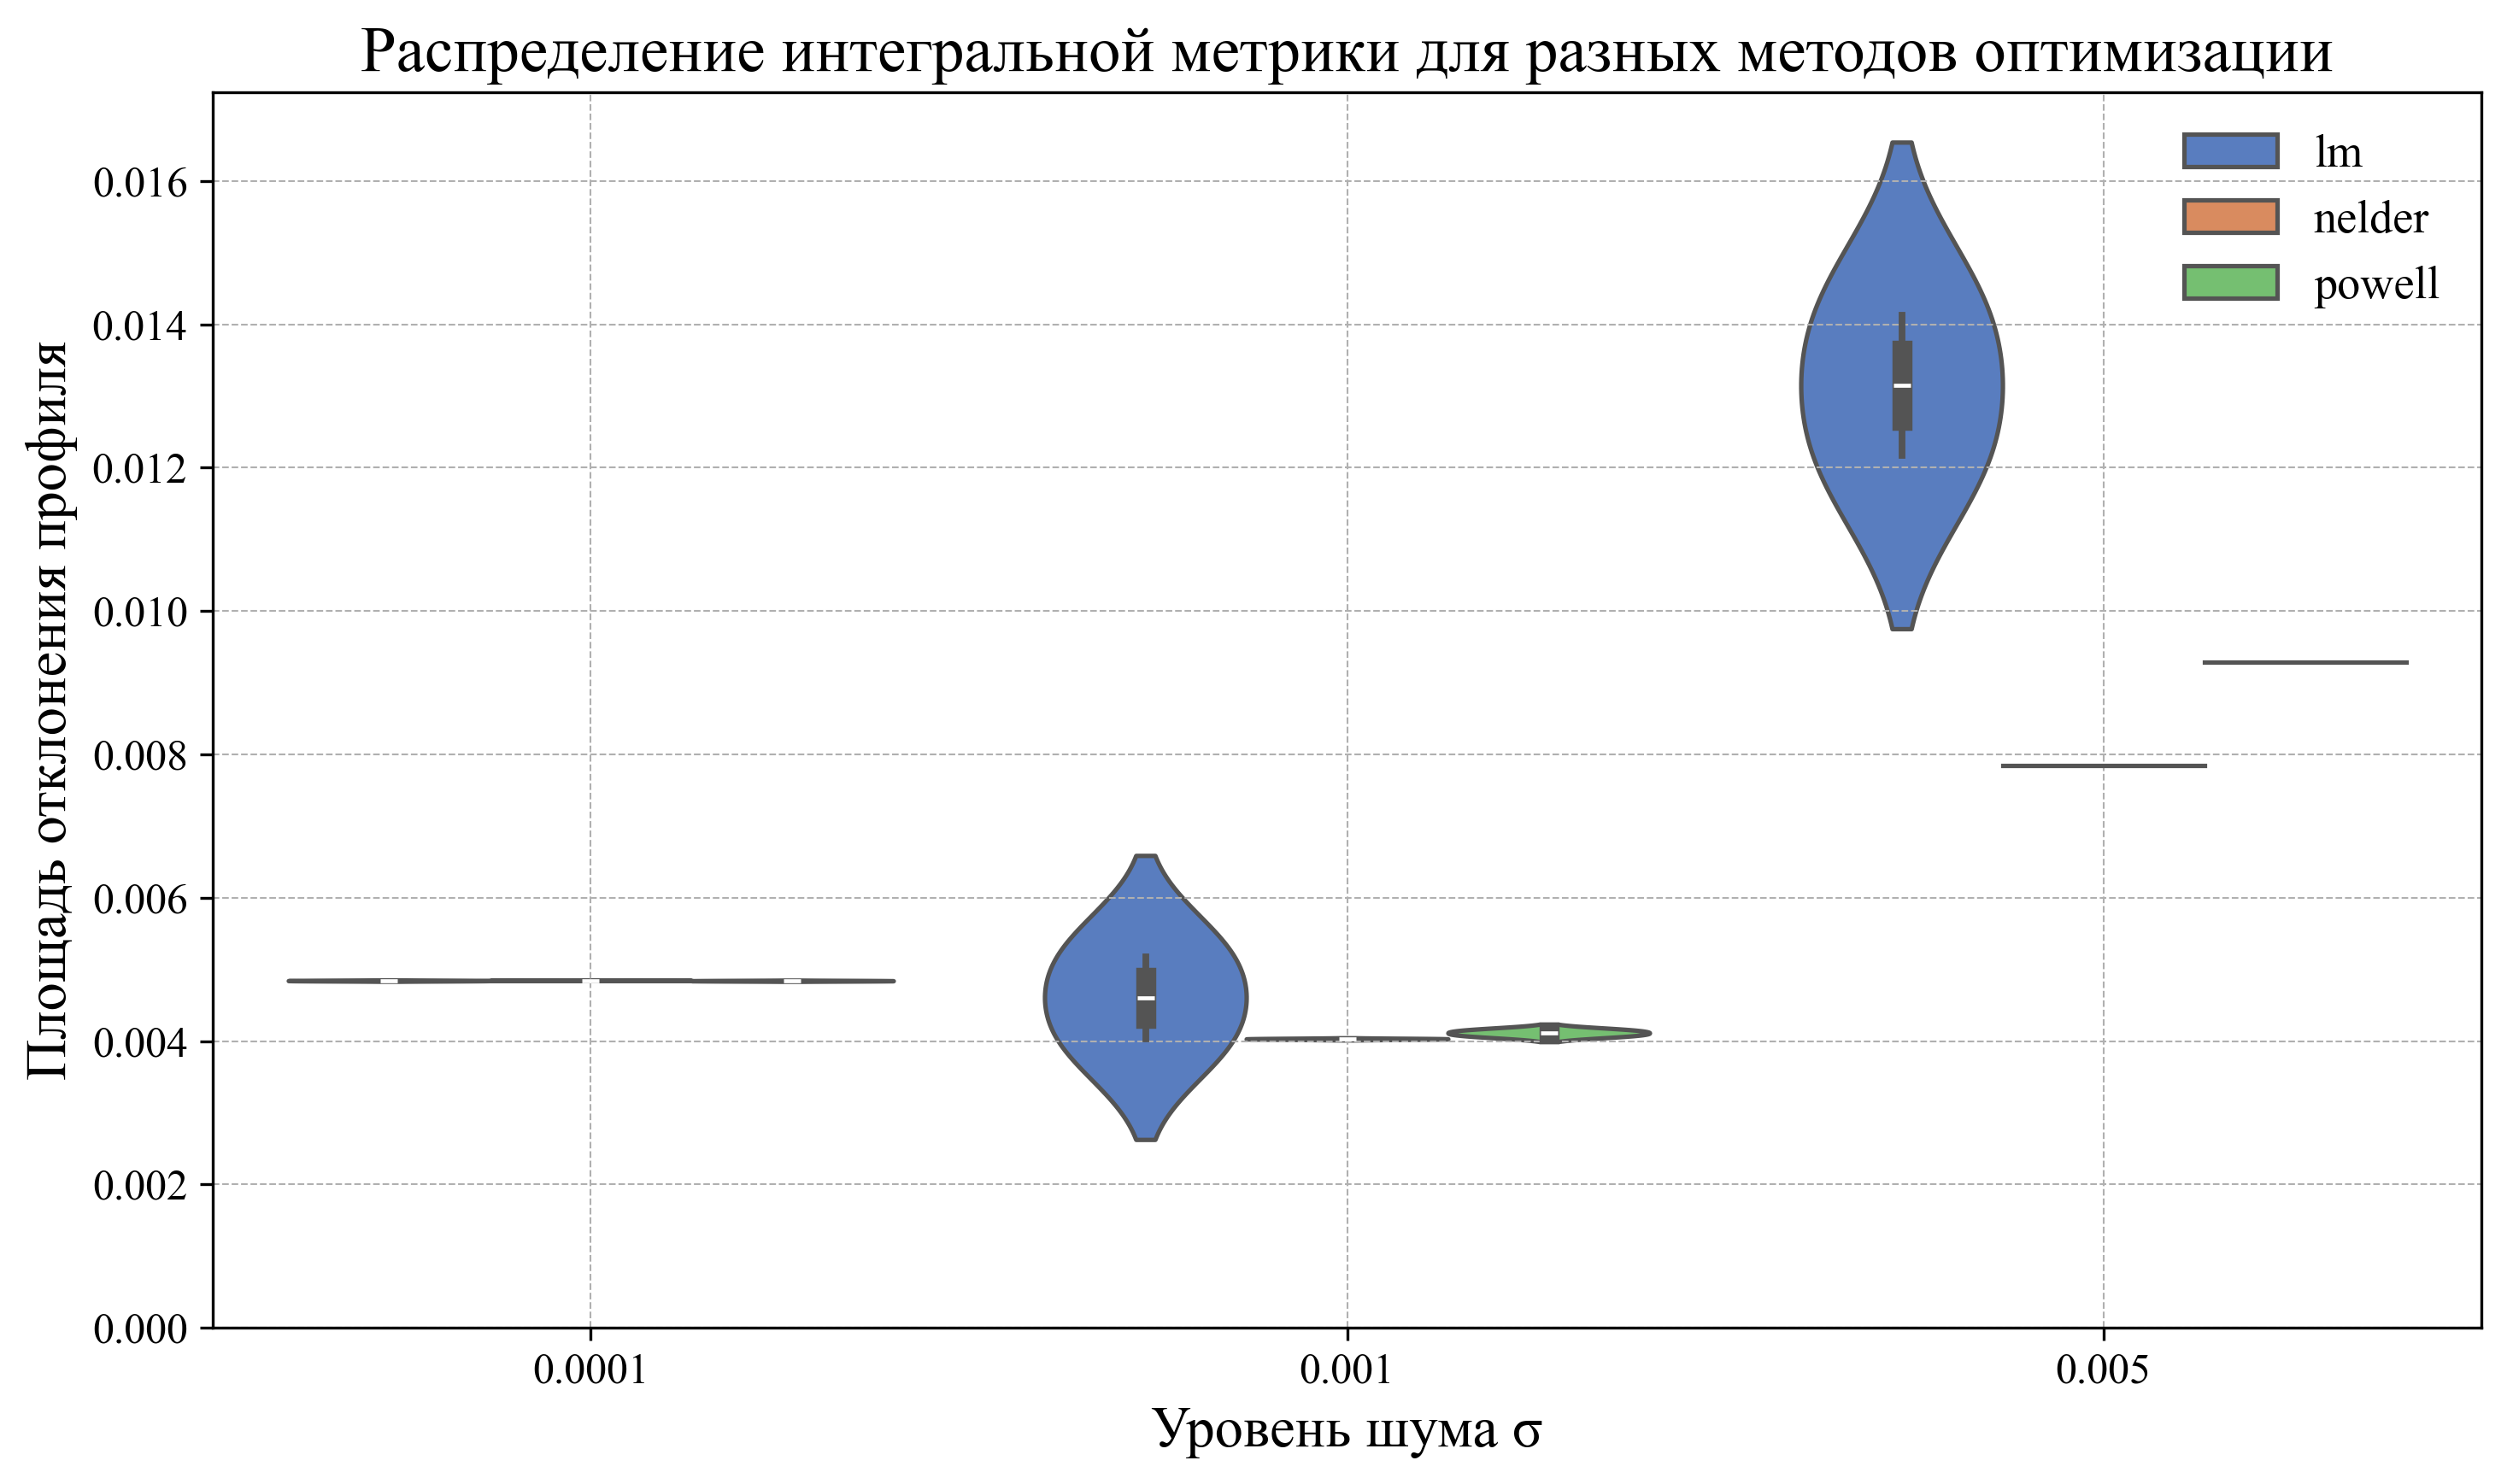
\includegraphics[width=\linewidth]{/Users/macbookmike_1/PycharmProjects/PythonProject/stability_tests/data/charts/stability_N_samples/violinplot_graph}
    \end{minipage}
\end{center}

Здесь аналогичная картина.

\section*{Карта применимости}
    Построена карта применимости модели по заданному уровню шума и значениям параметров A и Pe на первом изолированном интервале.
    (Пока только по 1 реализации шума для каждой комбинации A и Pe, поэтому карта такая неоднородная)

\begin{center}
    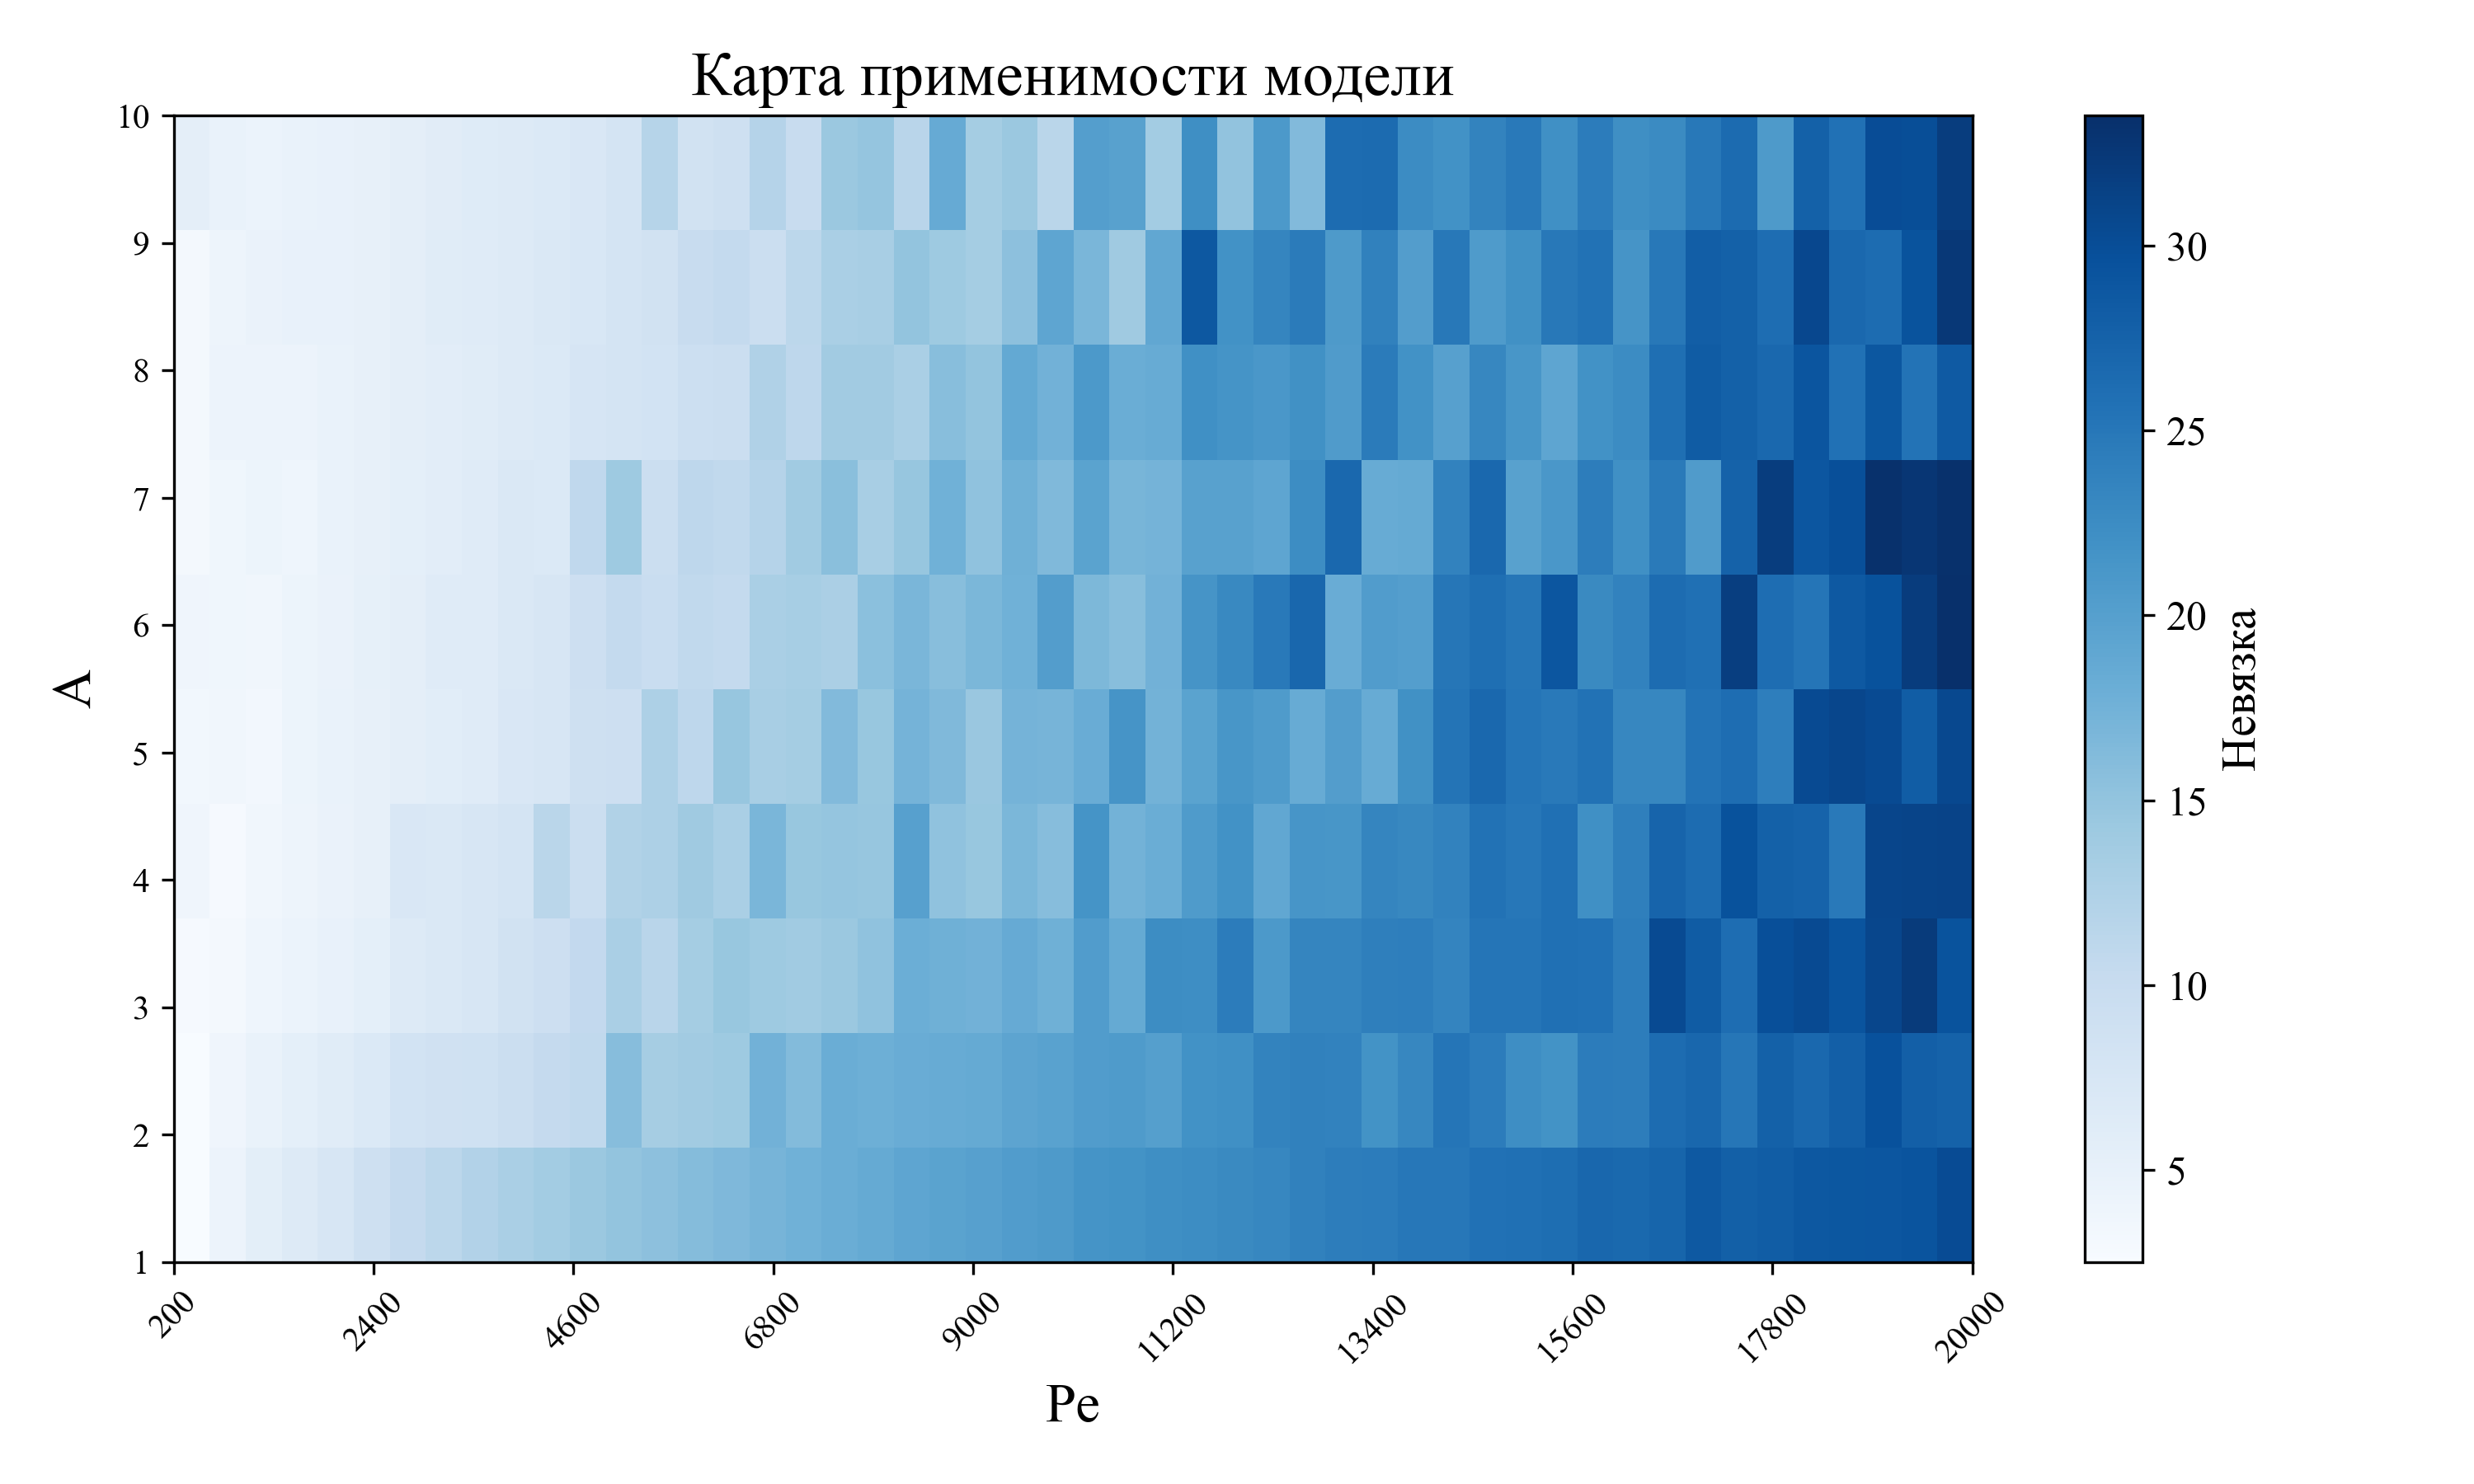
\includegraphics[width=0.85\textwidth]{/Users/macbookmike_1/PycharmProjects/PythonProject/stability_tests/data/charts/stability_applicability_map/applicability_map_heatmap}
\end{center}
\end{document}